% !TeX program = xelatex
% Author: Mark H. Olson
% Website: https://mholson.com
% Github: https://github.com/mholson

%=+=+=+=+=+=+=+=+=+=+=+=+=+=+=+=+=+=+=+=+=+=+=+=+=+=+=+=+=+=+=+=+=+=+=+=+=+=+=+=

%=-=-=-=-=-=-=-=-=-=-=-=-=-=-=-=-=-=-=-=-=-=-=-=-=-=-=-=-=-=-=-=-=-=-=-=-=-=-=-=
% PREAMBLE :: sthlmNordLightDemo.tex 
%=-=-=-=-=-=-=-=-=-=-=-=-=-=-=-=-=-=-=-=-=-=-=-=-=-=-=-=-=-=-=-=-=-=-=-=-=-=-=-=
%
% > > >	The following beamer class options are available
%		aspectratio=169		Change aspect ratio to 16:9	
%		bibref				Include bibliography
%		sectionpages		Show section pages
%		codeminted			use minted pkg for code printing instead of listings
%							(requires additional setup & Python installed)
% 		font sizes 			{8, 9, 10, 11, 12, 14, 17, 20} 11 Default
%
% > > > The following sthlmnord package options are available
%		mode				= dark (default)
%							= light
%=-=-=-=-=-=-=-=-=-=-=-=-=-=-=-=-=-=-=-=-=-=-=-=-=-=-=-=-=-=-=-=-=-=-=-=-=-=-=-=

\documentclass[usenames,11,dvipsnames,svgnames,x11names,aspectratio=1610,bibref]{beamer}
% > > > Bibliography File 
\newcommand{\bibfilename}{mhoreferences.bib}
% > > > Choose Theme
\usetheme[mode=light]{sthlmnord}
%\usetheme{sthlmnord}

\usepackage[normalem]{ulem}                 % \uline
\usepackage{multicol}
\usepackage{tikz}
\usepackage{stackengine}
\usepackage{xspace}
\usepackage{awesomebox}
% \usepackage[font=scriptsize,labelfont=bf]{caption}
\usepackage{subcaption} % for captionof
% \usepackage{cleveref}

% \usepackage{titlesec} % paragraph symbol \S
\usepackage{underscore}                     % to write underscores without escaping them
\usepackage[minted,listings]{tcolorbox}     % listing
\usepackage{minted}

\usemintedstyle{tango}
\usepackage{xparse}

\usepackage{paralist}                       % compactitem, compactenum


\usepackage{fontawesome5}

\newcommand{\cmark}{\ding{51}}%
\newcommand{\xmark}{\ding{55}}%


\newcommand{\myimportantbox}[1]{%
  \awesomebox[nordEleven]{2pt}{\faFire}{nordEleven}{#1}}
  
\newcommand{\mytipbox}[1]{%
  \awesomebox[nordEleven!50]{2pt}{\faLightbulb[regular]}{Tomato}{#1}}

%%%%%%%%%%%%%%%%%%%%%%%%%%%%%%%%%%%
% FONTS
%%%%%%%%%%%%%%%%%%%%%%%%%%%%%%%%%%%
\newfontfamily{\orbitron}{orbitron}[
    Path=./fonts/orbitron/,
    Extension = .otf,
    UprightFont = *-light,
    BoldFont = *-medium
    ]
    
\newfontfamily{\robotomono}{robotomono}[
    Path=./fonts/robotomono/,
    Extension = .ttf,
    UprightFont = *-Regular,
    BoldFont = *-Bold,
    BoldItalicFont = *-BoldItalic,
    ItalicFont = *-Italic,
    NFSSFamily=RobotoMonoFamily
    ]

% \newfontfamily\monaco{Arial}[NFSSFamily=ArialFamily]
% \setminted[matlab]{fontfamily=ArialFamily}

% \newfontfamily{\raleway}{Raleway}[
%     Path=./fonts/raleway/,
%     Extension = .ttf,
%     UprightFont = *-Medium,
%     BoldFont = *-Bold,
%     BoldItalicFont = *-BoldItalic,
%     ItalicFont = *-Italic
%     ]


    
    
    
% \newfontfamily{\ralewayII}{Raleway}[
%     Path=./fonts/raleway/,
%     Extension = .ttf,
%     UprightFont = *-Light,
%     BoldFont = *-SemiBold,
%     BoldItalicFont = *-SemiBoldItalic,
%     ItalicFont = *-LightItalic
%     ]

% \newfontfamily{\ralewayIII}{Raleway}[
%     Path=./fonts/raleway/,
%     Extension = .ttf,
%     UprightFont = *-Thin,
%     BoldFont = *-Bold,
%     BoldItalicFont = *-BoldItalic,
%     ItalicFont = *-Italic
%     ]
    


%%%%%%%%%%%%%%%%%%%%%%%%%%%%%%%%%%%
% code error
%%%%%%%%%%%%%%%%%%%%%%%%%%%%%%%%%%%
\definecolor{coderror}{HTML}{f06b6b}
\newcommand{\codeerror}{\textcolor{coderror}{\bf error}}
\newcommand{\codeerrorII}[1]{\textcolor{coderror}{\bf #1}}
%%%%%%%%%%%%%%%%%%%%%%%%%%%%%%%%%%%
% VINIK24 colors
%%%%%%%%%%%%%%%%%%%%%%%%%%%%%%%%%%%


% 000000
% 6f6776
% 9a9a97
% c5ccb8
% 8b5580
% c38890
% a593a5
% 666092
% 9a4f50
% c28d75
% 7ca1c0
% 416aa3
% 8d6268
% be955c
% 68aca9
% 387080
% 6e6962
% 93a167
% 6eaa78
% 557064
% 9d9f7f
% 7e9e99
% 5d6872
% 433455

\definecolor{vinik1}{HTML}{000000}
\newcommand{\vinikI}[1]{\textcolor{vinik1}{#1}}
\definecolor{vinik2}{HTML}{6f6776}
\newcommand{\vinikII}[1]{\textcolor{vinik2}{#1}}
\definecolor{vinik3}{HTML}{9a9a97}
\newcommand{\vinikIII}[1]{\textcolor{vinik3}{#1}}
\definecolor{vinik4}{HTML}{c5ccb8}
\newcommand{\vinikIV}[1]{\textcolor{vinik4}{#1}}
\definecolor{vinik5}{HTML}{8b5580}
\newcommand{\vinikV}[1]{\textcolor{vinik5}{#1}}
\definecolor{vinik6}{HTML}{c38890}
\newcommand{\vinikVI}[1]{\textcolor{vinik6}{#1}}
\definecolor{vinik7}{HTML}{a593a5}
\newcommand{\vinikVII}[1]{\textcolor{vinik7}{#1}}
\definecolor{vinik8}{HTML}{666092}
\newcommand{\vinikVIII}[1]{\textcolor{vinik8}{#1}}
\definecolor{vinik9}{HTML}{9a4f50}
\newcommand{\vinikIX}[1]{\textcolor{vinik9}{#1}}
\definecolor{vinik10}{HTML}{c28d75}
\newcommand{\vinikX}[1]{\textcolor{vinik10}{#1}}
\definecolor{vinik11}{HTML}{7ca1c0}
\newcommand{\vinikXI}[1]{\textcolor{vinik11}{#1}}
\definecolor{vinik12}{HTML}{416aa3}
\newcommand{\vinikXII}[1]{\textcolor{vinik12}{#1}}
\definecolor{vinik13}{HTML}{8d6268}
\newcommand{\vinikXIII}[1]{\textcolor{vinik13}{#1}}
\definecolor{vinik14}{HTML}{be955c}
\newcommand{\vinikXIV}[1]{\textcolor{vinik14}{#1}}
\definecolor{vinik15}{HTML}{68aca9}
\newcommand{\vinikXV}[1]{\textcolor{vinik15}{#1}}
\definecolor{vinik16}{HTML}{387080}
\newcommand{\vinikXVI}[1]{\textcolor{vinik16}{#1}}
\definecolor{vinik17}{HTML}{6e6962}
\newcommand{\vinikXVII}[1]{\textcolor{vinik17}{#1}}
\definecolor{vinik18}{HTML}{93a167}
\newcommand{\vinikXVIII}[1]{\textcolor{vinik18}{#1}}
\definecolor{vinik19}{HTML}{6eaa78}
\newcommand{\vinikXIX}[1]{\textcolor{vinik19}{#1}}
\definecolor{vinik20}{HTML}{557064}
\newcommand{\vinikXX}[1]{\textcolor{vinik20}{#1}}
\definecolor{vinik21}{HTML}{9d9f7f}
\newcommand{\vinikXXI}[1]{\textcolor{vinik21}{#1}}
\definecolor{vinik22}{HTML}{7e9e99}
\newcommand{\vinikXXII}[1]{\textcolor{vinik22}{#1}}
\definecolor{vinik23}{HTML}{5d6872}
\newcommand{\vinikXXIII}[1]{\textcolor{vinik23}{#1}}
\definecolor{vinik24}{HTML}{433455}
\newcommand{\vinikXXIV}[1]{\textcolor{vinik24}{#1}}

\newcommand{\syntaxgray}[1]{\textcolor{vinik23}{#1}}


\definecolor{definitioncolor}{HTML}{3C415C}
\newcommand{\mydefinitioncolor}[1]{\textcolor{definitioncolor}{#1}}



\definecolor{sectionchevron}{HTML}{76BA99}
\newcommand{\sectionColor}[1]{\textcolor{sectionchevron}{#1}}

\definecolor{subsectionchevron}{HTML}{ADCF9F}
\newcommand{\subsectionColor}[1]{\textcolor{subsectionchevron}{#1}}

\definecolor{subsubsectionchevron}{HTML}{CED89E}
\newcommand{\subsubsectionColor}[1]{\textcolor{subsubsectionchevron}{#1}}

\definecolor{customcolor}{HTML}{A77979}
\definecolor{citationcolor}{HTML}{F67280}
\newcommand{\citationcolor}[1]{\textcolor{nordEleven}{#1}}




%%%%%%%%%%%%%%%%%%%%%%%%%%%%%%%%%%%
% CARNIVAL32 colors
%%%%%%%%%%%%%%%%%%%%%%%%%%%%%%%%%%%


% 000000
% 6f6776
% 9a9a97
% c5ccb8
% 8b5580
% c38890
% a593a5
% 666092
% 9a4f50
% c28d75
% 7ca1c0
% 416aa3
% 8d6268
% be955c
% 68aca9
% 387080
% 6e6962
% 93a167
% 6eaa78
% 557064
% 9d9f7f
% 7e9e99
% 5d6872
% 433455

\definecolor{carnival19}{HTML}{4d528a}
\newcommand{\carnivalXIX}[1]{\textcolor{carnival19}{#1}}
\newcommand{\monster}{\textbf{\textcolor{DodgerBlue1}{rpg::Monster}}}
\newcommand{\vampire}{\textbf{\textcolor{BurntOrange}{rpg::Vampire}}}
\newcommand{\werewolf}{\textbf{\textcolor{WildStrawberry}{rpg::Werewolf}}}


\definecolor{carnival20}{HTML}{556a97}
\newcommand{\carnivalXX}[1]{\textcolor{carnival20}{#1}}




\definecolor{carnival21}{HTML}{5c81a3}
\newcommand{\carnivalXXI}[1]{\textcolor{carnival21}{#1}}
\definecolor{carnival22}{HTML}{7dadc8}
\newcommand{\carnivalXXII}[1]{\textcolor{carnival22}{#1}}
\definecolor{carnival23}{HTML}{b0d6d9}
\newcommand{\carnivalXXIII}[1]{\textcolor{carnival23}{#1}}
\definecolor{carnival24}{HTML}{ece6df}
\newcommand{\carnivalXXIV}[1]{\textcolor{carnival24}{#1}}
\definecolor{carnival25}{HTML}{cfccca}
\newcommand{\carnivalXXV}[1]{\textcolor{carnival25}{#1}}




\definecolor{iconColor}{HTML}{383E56}
\definecolor{iconWarningColor}{HTML}{FA370E}
\definecolor{iconOkColor}{HTML}{00A8CC}
\definecolor{iconBestPracticeColor}{HTML}{00A8CC}
\newcommand{\iconColor}[1]{\textcolor{iconColor}{#1}}
\newcommand{\iconWarningColor}[1]{\textcolor{iconWarningColor}{#1}}
\newcommand{\iconBestPracticeColor}[1]{\textcolor{DodgerBlue}{#1}}

\newcommand{\iconOKColor}[1]{\textcolor{iconOkColor}{#1}}

\definecolor{codecolor1}{HTML}{004822}
\newcommand{\codecolorI}[1]{\textcolor{DeepPink1}{\bf #1}}
\definecolor{codecolor2}{HTML}{FD3135}
\newcommand{\codecolorII}[1]{\textcolor{DeepSkyBlue4}{\bf #1}}
\definecolor{codecolor3}{HTML}{0E6B8C}
\newcommand{\codecolorIII}[1]{\textcolor{IndianRed1}{\bf #1}}


\newcommand{\crosmsgComment}[1]{{\color{nordThree}{\textit{#1}}}}
\definecolor{disclaimer}{HTML}{EBCB8B}  
\newcommand{\mydisclaimer}{{\color{disclaimer}{\footnotesize Lecture 5~}}}
%%%%%%%%%%%%%%%%%%%%%%%%%%%%%%%%%%%
% line number customized
\renewcommand{\theFancyVerbLine}{\textcolor{carnival19}{\sf\scriptsize\arabic{FancyVerbLine}}}
\newcommand{\myline}[1]{{\textcolor{carnival19}{#1}}}
%%%%%%%%%%%%%%%%%%%%%%%%%%%%%%%%%%%

%%%%%%%%%%%%%%%%%%%%%%%%%%%%%%%%%%%
% Directory tree
%%%%%%%%%%%%%%%%%%%%%%%%%%%%%%%%%%%
\usepackage[edges]{forest}

\newlength\Size
\setlength\Size{4pt}
\tikzset{%
  folder/.pic={%
  \node[inner sep=0pt] (folder) at (0.16,0)
    {\normalsize\textcolor{black}{\faFolderOpen}};
    % \filldraw [draw=folderborder, top color=folderbg!50, bottom color=folderbg] (-1.05*\Size,0.2\Size+5pt) rectangle ++(.75*\Size,-0.2\Size-5pt);
    % \filldraw [draw=folderborder, top color=folderbg!50, bottom color=folderbg] (-1.15*\Size,-\Size) rectangle (1.15*\Size,\Size);
  },
  file/.pic={%
  \node[inner sep=0pt] (file) at (0.13,0)
    {\normalsize\faFile*[regular]};
    % \filldraw [draw=folderborder, top color=folderbg!5, bottom color=folderbg!10] (-\Size,.4*\Size+5pt) coordinate (a) |- (\Size,-1.2*\Size) coordinate (b) -- ++(0,1.6*\Size) coordinate (c) -- ++(-5pt,5pt) coordinate (d) -- cycle (d) |- (c) ;
  },
}
\forestset{%
  declare autowrapped toks={pic me}{},
  declare boolean register={pic root},
  pic root=0,
  pic dir tree/.style={%
    for tree={%
      folder,
      font=\raleway,
      grow'=0,
      l=0,
    },
    before typesetting nodes={%
      for tree={%
        edge label+/.option={pic me},
        l=0,
      },
      if pic root={
        tikz+={
          \pic at ([xshift=\Size].west) {folder};
        },
        align={l}
      }{},
    },
  },
  pic me set/.code n args=2{%
    \forestset{%
      #1/.style={%
        inner xsep=10,
        pic me={pic {#2}},
      }
    }
  },
  pic me set={directory}{folder},
  pic me set={file}{file},
}



%%%%%%%%%%%%%%%%%%%%%%%%%%%%%%%%%%%
% Stuff for table of contents
%%%%%%%%%%%%%%%%%%%%%%%%%%%%%%%%%%%
\usetikzlibrary{positioning}
\usetikzlibrary{tikzmark}
\tikzset{
  section number/.style={
    draw=none,
    rectangle,    
    left color=nordZero,
    right color=nordZero,
    minimum size=1.5em,
    text=white,
  },
  section/.style={
    draw=none,
    rectangle,    
    % shading=section shading,
    minimum height=1.5em,
    minimum width=0.9\textwidth,
    text width=0.9\textwidth,
    text=black,
    align=left
  },
  subsection number/.style={
    draw=none,
    rectangle,    
    left color=nordTwo,
    right color=nordTwo,
    minimum size=0.5em,
    text=white,
  },
  subsection/.style={
    draw=none,
    rectangle,    
    % shading=subsection shading,
    minimum height=1.5em,
    minimum width=0.939\textwidth,
    text width=0.939\textwidth,
    text=black,
    align=left
  }
}

\setbeamertemplate{section in toc}{
    \tikz[baseline=-0.5ex]\node[section number]{\,\inserttocsectionnumber};%
  \,%
  \tikz[baseline=-0.5ex]\node[section]{\inserttocsection};
}
\setbeamertemplate{subsection in toc}{
\tikz[baseline=-0.5ex]\node[subsection number]{\,\inserttocsubsectionnumber};%
  \,%
  \tikz[baseline=-0.5ex]\node[subsection]{\inserttocsubsection};
}

%%%%%%%%%%%%%%%%%%%%%%%%%%%%%%%%%%%
% href stuff
%%%%%%%%%%%%%%%%%%%%%%%%%%%%%%%%%%%
\newcommand{\urllink}[2]{\href{#1}{\textcolor{DimGray}{\uline{#2}}}}

\newcommand{\myemail}[2]{\href{#1}{\cnordTwelve{{\scriptsize\faEnvelope[regular]~}\uline{#2}}}}
%%%%%%%%%%%%%%%%%%%%%%%%%%%%%%%%%%%
% listing
%%%%%%%%%%%%%%%%%%%%%%%%%%%%%%%%%%%
\tcbuselibrary{listings, minted, skins}
\tcbset{listing engine=minted}


%%%%%%%%%%%%%%%%%%%%%%%%%%%%%%%%%%%
% sec, secsec, secsecsec
%%%%%%%%%%%%%%%%%%%%%%%%%%%%%%%%%%%
\newcommand\myhrulefill{\cnordTen{\hrulefill}}
\newcommand\myhrulefillred{\cnordEleven{\hrulefill}}
% Configure style for custom doubled line
\newcommand*{\doublerule}{\hrule width \hsize height 1pt \kern 0.5mm \hrule width \hsize height 2pt}

% Configure function to fill line with doubled line
\newcommand\doublerulefill{\leavevmode\leaders\vbox{\hrule width .1pt\kern1pt\hrule}\hfill\kern0pt }

% \newcommand{\mydisclaimer}{\cnordTwelve{Disclaimer}}
\renewcommand\sec{{\cnordSix{\secname}\hfill\mydisclaimer} }

\newcommand\secsec{\cnordSix{\secname}~\sectionColor{\small\faChevronRight}~{\cnordFive{\small\subsecname}\hfill\mydisclaimer}}

\newcommand\secsecsec{\cnordSix{\secname}~\sectionColor{\small\faChevronRight}~{\cnordFive{\small\subsecname}}~\subsectionColor{\footnotesize\faChevronRight}~{\cnordFour{\footnotesize\subsubsecname}\hfill\mydisclaimer}}

\newcommand\secsecsecsec[1]{\cnordSix{\secname}~\sectionColor{\small\faChevronRight}~{\cnordFive{\small\subsecname}}~\subsectionColor{\footnotesize\faChevronRight}~{\cnordFour{\footnotesize\subsubsecname}}~\subsubsectionColor{\scriptsize\faChevronRight}~{\cnordFour{\scriptsize #1}\hfill\mydisclaimer}}


%%%%%%%%%%%%%%%%%%%%%%%%%%%%%%%%%%%%%%%%%%%%%%%%%%%%%%%
\newcommand{\myDefinitionIcon}{\iconColor{\faScroll}\xspace}
% \newcommandx{\myDefinitionHeader}[3][1=12pt, 2=12pt]{{\fontsize{#1}{#2}\selectfont \myDefinitionIcon #3} \doublerulefill}

% \newcommand{\myDefinitionHeader}[3][12pt]{\fontsize{#2}{#1}\selectfont #3}


% \newcommand\secsecsec{{\color{darkgray}{\normalsize{\secname}} \textcolor{Tomato3}{|}{{\color{darkgray!90}{\small\subsecname}}}\textcolor{Tomato3}{|}{\color{darkgray!70}{\footnotesize\subsubsecname}}\myhrulefill}}



    
%%%%%%%%%%%%%%%%%%%%%%%%%%%%%%%%%%%
% C++
%%%%%%%%%%%%%%%%%%%%%%%%%%%%%%%%%%%
\def\CC{{C\nolinebreak[4]\hspace{-.05em}\raisebox{.4ex}{\tiny\bf ++}}\xspace}

\def\CCNINETYEIGHT{{C\nolinebreak[4]\hspace{-.05em}\raisebox{.4ex}{\tiny\bf ++98}}\xspace}
\def\CNINETYNINE{{C\nolinebreak[4]\hspace{-.05em}\raisebox{.4ex}{\tiny\bf 99}}\xspace}
\def\CCZEROTHREE{{C\nolinebreak[4]\hspace{-.05em}\raisebox{.4ex}{\tiny\bf ++03}}\xspace}
\def\CCELEVEN{{C\nolinebreak[4]\hspace{-.05em}\raisebox{.4ex}{\tiny\bf ++11}}\xspace}
\def\CCFOURTEEN{{C\nolinebreak[4]\hspace{-.05em}\raisebox{.4ex}{\tiny\bf ++14}}\xspace}
\def\CCSEVENTEEN{{C\nolinebreak[4]\hspace{-.05em}\raisebox{.4ex}{\tiny\bf ++17}}\xspace}
\def\CCTWENTY{{C\nolinebreak[4]\hspace{-.05em}\raisebox{.4ex}{\tiny\bf ++20}}\xspace}
\def\SALARY{{Salary\nolinebreak[4]\hspace{-.05em}\raisebox{.4ex}{\tiny\bf ++}}\xspace}


%%%%%%%%%%%%%%%%%%%%%%%%%%%%%%%%%%%%%%%%%%%%%%
\newmintinline[mfoot]{cpp}{fontsize=\footnotesize, fontfamily=RobotoMonoFamily, escapeinside=||}
\newmintinline[pfoot]{python}{fontsize=\footnotesize, fontfamily=RobotoMonoFamily, escapeinside=||}
\newmintinline[mlarge]{cpp}{fontsize=\large,fontfamily=RobotoMonoFamily, escapeinside=||}
\newmintinline[mLarge]{cpp}{fontsize=\Large,fontfamily=RobotoMonoFamily, escapeinside=||}
\newmintinline[mhuge]{cpp}{fontsize=\huge,fontfamily=RobotoMonoFamily, escapeinside=||}
\newmintinline[mHuge]{cpp}{fontsize=\Huge,fontfamily=RobotoMonoFamily, escapeinside=||}
\newmintinline[msmall]{cpp}{fontsize=\small,fontfamily=RobotoMonoFamily, escapeinside=||}
\newmintinline[mnormal]{cpp}{fontsize=\fontsize{11}{12}\selectfont, fontfamily=RobotoMonoFamily,escapeinside=||}

\newmintinline[pnormal]{python}{fontsize=\fontsize{11}{12}\selectfont, fontfamily=RobotoMonoFamily, escapeinside=||}

\newmintinline[mscript]{cpp}{fontsize=\scriptsize,fontfamily=RobotoMonoFamily, escapeinside=||}

\newmintinline[pscript]{python}{fontsize=\scriptsize, fontfamily=RobotoMonoFamily, escapeinside=||}


\newmintinline[mtiny]{cpp}{fontsize=\tiny,fontfamily=RobotoMonoFamily, escapeinside=||}

%%%%%%%%%%%%%%%%%%%% BASH
\newcommand\bashNormal[1]{{\mintinline[fontsize=\normalsize]{bash}{#1}}}
\newcommand\bashSmall[1]{{\mintinline[fontsize=\small]{bash}{#1}}}
\newcommand\bashFootnote[1]{{\mintinline[fontsize=\fontsize{9}{11}\selectfont]{bash}{#1}}}
\newcommand\bashScript[1]{\mintinline[fontsize=\fontsize{7}{9}\selectfont]{bash}{#1}}




%%%%%%%%%%%%%%%%%%%%%%%%%%%%%%%%%%%%%%%%%%%%%%
\newtcblisting{cppscript}{listing only, 
    minted language=cpp, 
    % minted style=stata-light,
    minted style=tango,
    % minted bgcolor=\cnordSix,
    colback=white, enhanced, frame hidden,
    boxsep=0pt,top=-2.5mm,bottom=-2.5mm,left=-1mm,right=-1mm,
nobeforeafter,
    minted options={
    fontfamily=RobotoMonoFamily,
    bgcolor=white,
    fontsize=\scriptsize, 
    tabsize=1, 
    frame=leftline,
    escapeinside=||,
    rulecolor=nordFourteen,
    framerule=2pt,
    breaklines, 
    autogobble}
}


\newtcblisting{pyfoot}{listing only, 
    minted language=python, 
    % minted style=stata-light,
    minted style=tango,
    % minted bgcolor=\cnordSix,
    colback=white, enhanced, frame hidden,
    boxsep=0pt,top=-2.5mm,bottom=-2.5mm,left=-1mm,right=-1mm,
nobeforeafter,
    minted options={
    fontfamily=RobotoMonoFamily,
    bgcolor=white,
    fontsize=\footnotesize, 
    tabsize=1, 
    frame=leftline,
    escapeinside=||,
    rulecolor=Firebrick3,
    framerule=2pt,
    breaklines, 
    autogobble}
}

\newtcblisting{cmakescript}{listing only, 
    minted language=cmake, 
    minted style=tango,
    colback=white, enhanced, frame hidden,
    boxsep=0pt,top=-2.5mm,bottom=-2.5mm,left=-1mm,right=-1mm,
nobeforeafter,
    minted options={
    % fontfamily=FiraCode,
    fontfamily=RobotoMonoFamily,
    bgcolor=white,
    fontsize=\fontsize{7}{8}\selectfont, 
    tabsize=2, 
    frame=leftline,
    escapeinside=@@,
    rulecolor=nordZero,
    framerule=2pt,
    breaklines, 
    autogobble}
}


\newtcblisting{cmakefoot}{listing only, 
    minted language=cmake, 
    minted style=tango,
    colback=white, enhanced, frame hidden,
    boxsep=0pt,top=-2.5mm,bottom=-2.5mm,left=-1mm,right=-1mm,
nobeforeafter,
    minted options={
    % fontfamily=FiraCode,
    fontfamily=RobotoMonoFamily,
    bgcolor=white,
    fontsize=\fontsize{8}{9}\selectfont, 
    tabsize=2, 
    frame=leftline,
    escapeinside=@@,
    rulecolor=nordZero,
    framerule=2pt,
    breaklines, 
    autogobble}
}
%%%%%%%%%%%%%%%%%%%%%%%%%%%%%%%%%%%%%%%%%%%%%%
\newtcblisting{pyscript}{listing only, 
    minted language=python, 
    % minted style=stata-light,
    minted style=tango,
    % minted bgcolor=\cnordSix,
    colback=white, enhanced, frame hidden,
    boxsep=0pt,top=-2.5mm,bottom=-2.5mm,left=-1mm,right=-1mm,
nobeforeafter,
    minted options={
    fontfamily=RobotoMonoFamily,
    bgcolor=white,
    fontsize=\scriptsize, 
    tabsize=1, 
    frame=leftline,
    escapeinside=||,
    rulecolor=nordFourteen,
    framerule=2pt,
    breaklines, 
    autogobble}
}

%%%%%%%%%%%%%%%%%%%%%%%%%%%%%%%%%%%%%%%%%%%%%%
\newtcblisting{pyscriptII}{listing only, 
    minted language=python, 
    % minted style=stata-light,
    minted style=tango,
    % minted bgcolor=\cnordSix,
    colback=white, enhanced, frame hidden,
    boxsep=0pt,top=-2.5mm,bottom=-2.5mm,left=-1mm,right=-1mm,
nobeforeafter,
    minted options={
    fontfamily=RobotoMonoFamily,
    bgcolor=white,
    fontsize=\fontsize{7}{8}\selectfont, 
    tabsize=1, 
    frame=leftline,
    escapeinside=||,
    rulecolor=nordFourteen,
    framerule=2pt,
    breaklines, 
    autogobble}
}

%%%%%%%%%%%%%%%%%%%%%%%%%%%%%%%%%%%%%%%%%%%%%%
\newtcblisting{yamlscriptII}{listing only, 
    minted language=yaml, 
    % minted style=stata-light,
    minted style=tango,
    % minted bgcolor=\cnordSix,
    colback=white, enhanced, frame hidden,
    boxsep=0pt,top=-2.5mm,bottom=-2.5mm,left=-1mm,right=-1mm,
nobeforeafter,
    minted options={
    fontfamily=RobotoMonoFamily,
    bgcolor=white,
    fontsize=\fontsize{7}{8}\selectfont, 
    tabsize=1, 
    frame=leftline,
    escapeinside=||,
    rulecolor=nordFourteen,
    framerule=2pt,
    breaklines, 
    autogobble}
}
%%%%%%%%%%%%%%%%%%%%%%%%%%%%%%%%%%%%%%%%%%%%%%
\newtcblisting{xmlscript}{listing only, 
    minted language=xml, 
    % minted style=stata-light,
    minted style=tango,
    % minted bgcolor=\cnordSix,
    colback=white, enhanced, frame hidden,
    boxsep=0pt,top=-2.5mm,bottom=-2.5mm,left=-1mm,right=-1mm,
nobeforeafter,
    minted options={
    fontfamily=RobotoMonoFamily,
    bgcolor=white,
    fontsize=\scriptsize, 
    tabsize=1, 
    frame=leftline,
    escapeinside=||,
    rulecolor=nordThirteen,
    framerule=2pt,
    breaklines, 
    autogobble}
}

%%%%%%%%%%%%%%%%%%%%%%%%%%%%%%%%%%%%%%%%%%%%%%
\newtcblisting{xmlscriptII}{listing only, 
    minted language=xml, 
    % minted style=stata-light,
    minted style=tango,
    % minted bgcolor=\cnordSix,
    colback=white, enhanced, frame hidden,
    boxsep=0pt,top=-2.5mm,bottom=-2.5mm,left=-1mm,right=-1mm,
nobeforeafter,
    minted options={
    fontfamily=RobotoMonoFamily,
    bgcolor=white,
    fontsize=\fontsize{7}{8}\selectfont, 
    tabsize=1, 
    frame=leftline,
    escapeinside=||,
    rulecolor=nordThirteen,
    framerule=2pt,
    breaklines, 
    autogobble}
}

%%%%%%%%%%%%%%%%%%%%%%%%%%%%%%%%%%%%%%%%%%%%%%
\newtcblisting{xmltiny}{listing only, 
    minted language=xml, 
    % minted style=stata-light,
    minted style=tango,
    % minted bgcolor=\cnordSix,
    colback=white, enhanced, frame hidden,
    boxsep=0pt,top=-2.5mm,bottom=-2.5mm,left=-1mm,right=-1mm,
nobeforeafter,
    minted options={
    fontfamily=RobotoMonoFamily,
    bgcolor=white,
    fontsize=\tiny, 
    tabsize=1, 
    frame=leftline,
    escapeinside=||,
    rulecolor=nordThirteen,
    framerule=2pt,
    breaklines, 
    autogobble}
}


\newtcblisting{bashscript}{listing only, 
    minted language=bash, 
    % minted style=stata-light,
    minted style=tango,
    % minted bgcolor=\cnordSix,
    colback=white, enhanced, frame hidden,
    boxsep=0pt,top=-2.5mm,bottom=-2.5mm,left=-1mm,right=-1mm,
    nobeforeafter,
    minted options={
    fontfamily=RobotoMonoFamily,
    bgcolor=white,
    fontsize=\scriptsize, 
    tabsize=1, 
    frame=leftline,
    escapeinside=||,
    rulecolor=nordFourteen,
    framerule=2pt,
    breaklines, 
    autogobble}
}


\newtcblisting{bashfoot}{listing only, 
    minted language=bash, 
    % minted style=stata-light,
    minted style=tango,
    % minted bgcolor=\cnordSix,
    colback=white, enhanced, frame hidden,
    boxsep=0pt,top=-2.5mm,bottom=-2.5mm,left=-1mm,right=-1mm,
nobeforeafter,
    minted options={
    fontfamily=RobotoMonoFamily,
    bgcolor=nordSix,
    fontsize=\footnotesize, 
    tabsize=1, 
    frame=leftline,
    escapeinside=||,
    rulecolor=nordFourteen,
    framerule=2pt,
    breaklines, 
    autogobble}
}

\newtcblisting{textfoot}{listing only, 
    minted language=text, 
    % minted style=stata-light,
    minted style=tango,
    % minted bgcolor=\cnordSix,
    colback=white, enhanced, frame hidden,
    boxsep=0pt,top=-2.5mm,bottom=-2.5mm,left=-1mm,right=-1mm,
nobeforeafter,
    minted options={
    fontfamily=RobotoMonoFamily,
    bgcolor=white,
    fontsize=\footnotesize, 
    tabsize=1, 
    frame=leftline,
    escapeinside=||,
    rulecolor=DeepSkyBlue4,
    framerule=2pt,
    breaklines, 
    autogobble}
}

\newtcblisting{textscript}{listing only, 
    minted language=text, 
    minted style=stata-light,
    % minted style=tango,
    % minted bgcolor=\cnordSix,
    colback=white, enhanced, frame hidden,
    boxsep=0pt,top=-2.5mm,bottom=-2.5mm,left=-1mm,right=-1mm,
nobeforeafter,
    minted options={
    fontfamily=RobotoMonoFamily,
    bgcolor=white,
    fontsize=\fontsize{7}{9}\selectfont, 
    tabsize=1, 
    frame=leftline,
    escapeinside=||,
    rulecolor=DeepSkyBlue4,
    framerule=2pt,
    breaklines, 
    autogobble}
}


\newtcblisting{yamlscript}{listing only, 
    minted language=yaml, 
    minted style=stata-light,
    % minted style=tango,
    % minted bgcolor=\cnordSix,
    colback=white, enhanced, frame hidden,
    boxsep=0pt,top=-2.5mm,bottom=-2.5mm,left=-1mm,right=-1mm,
nobeforeafter,
    minted options={
    fontfamily=RobotoMonoFamily,
    bgcolor=white,
    fontsize=\fontsize{7}{9}\selectfont, 
    tabsize=1, 
    frame=leftline,
    escapeinside=||,
    rulecolor=Coral2,
    framerule=2pt,
    breaklines, 
    autogobble}
}

\newtcblisting{texttiny}{listing only, 
    minted language=text, 
    minted style=stata-light,
    % minted style=tango,
    % minted bgcolor=\cnordSix,
    colback=white, enhanced, frame hidden,
    boxsep=0pt,top=-2.5mm,bottom=-2.5mm,left=-1mm,right=-1mm,
nobeforeafter,
    minted options={
    fontfamily=RobotoMonoFamily,
    bgcolor=white,
    fontsize=\tiny, 
    tabsize=1, 
    frame=leftline,
    escapeinside=||,
    rulecolor=DeepSkyBlue4,
    framerule=2pt,
    breaklines, 
    autogobble}
}


\newtcblisting{cppscriptII}{listing only, 
    minted language=cpp, 
    % minted style=stata-light,
    minted style=tango,
    % minted bgcolor=\cnordSix,
    colback=white, enhanced, frame hidden,
    boxsep=0pt,top=-2.5mm,bottom=-2.5mm,left=-1mm,right=-1mm,
nobeforeafter,
    minted options={
    fontfamily=RobotoMonoFamily,
    bgcolor=white,
    fontsize=\fontsize{7}{8}\selectfont, 
    tabsize=1, 
    frame=leftline,
    escapeinside=||,
    rulecolor=nordFourteen,
    framerule=2pt,
    breaklines, 
    autogobble}
}


\newtcblisting{cppscriptIILine}{listing only, 
    minted language=cpp, 
    % minted style=stata-light,
    minted style=tango,
    % minted bgcolor=\cnordSix,
    colback=white, enhanced, frame hidden,
    boxsep=0pt,top=-2.5mm,bottom=-2.5mm,left=-1mm,right=-1mm,
nobeforeafter,
    minted options={
    fontfamily=RobotoMonoFamily,
    bgcolor=white,
    fontsize=\fontsize{7}{8}\selectfont, 
    tabsize=1, 
    frame=leftline,
    linenos,
    escapeinside=||,
    rulecolor=nordFourteen,
    framerule=2pt,
    breaklines, 
    autogobble}
}





\newtcblisting{cppscriptline}{listing only, 
    minted language=cpp, 
    minted style=tango,
    % minted bgcolor=\cnordSix,
    colback=white, enhanced, frame hidden,
    boxsep=0pt,top=-2.5mm,bottom=-2.5mm,left=-1mm,right=-1mm,
nobeforeafter,
    minted options={
    fontfamily=RobotoMonoFamily,
    bgcolor=nordSix,
    fontsize=\scriptsize, 
    tabsize=1, 
    frame=leftline,
    linenos,
    escapeinside=||,
    rulecolor=nordFourteen,
    framerule=2pt,
    breaklines, 
    autogobble}
}

\newtcblisting{cppscriptlineTwoFive}{listing only, 
    minted language=cpp, 
    minted style=tango,
    % minted bgcolor=\cnordSix,
    colback=white, enhanced, frame hidden,
    boxsep=0pt,top=-2.5mm,bottom=-2.5mm,left=-1mm,right=-1mm,
nobeforeafter,
    minted options={
    fontfamily=RobotoMonoFamily,
    bgcolor=nordSix,
    highlightlines={2, 5},
    highlightcolor=nordThirteen,
    fontsize=\scriptsize, 
    tabsize=1, 
    frame=leftline,
    escapeinside=||,
    rulecolor=nordFourteen,
    framerule=2pt,
    breaklines, 
    linenos,
    autogobble}
}

\newtcblisting{textline}{listing only, 
    minted language=text, 
    minted style=tango,
    % minted bgcolor=\cnordSix,
    colback=white, enhanced, frame hidden,
    boxsep=0pt,top=-2.5mm,bottom=-2.5mm,left=-1mm,right=-1mm,
nobeforeafter,
    minted options={
    bgcolor=nordSix,
    fontsize=\scriptsize, 
    tabsize=1, 
    frame=leftline,
    linenos,
    escapeinside=||,
    rulecolor=nordFourteen,
    framerule=2pt,
    breaklines, 
    autogobble}
}


\newtcblisting{cppnormal}{listing only, 
    minted language=cpp, 
    minted style=tango,
    % minted bgcolor=\cnordSix,
    colback=white, enhanced, frame hidden,
    boxsep=0pt,top=-2.5mm,bottom=-2.5mm,left=-1mm,right=-1mm,
    nobeforeafter,
    minted options={
    fontfamily=RobotoMonoFamily,
    bgcolor=nordSix,
    fontsize=\normalsize, 
    tabsize=1, 
    frame=leftline,
    escapeinside=||,
    rulecolor=nordFourteen,
    framerule=2pt,
    breaklines, 
    autogobble}
}



\lstdefinelanguage{ROSMSG}{
    keywordstyle=\color{blue},
    keywordstyle = [2]{\color{VioletRed4}},
    keywordstyle = [3]{\color{OrangeRed1}},
    alsoletter=0123456789,
    alsodigit = {_},
    keywords={uint8,string,float32,float64, bool, int8},
    otherkeywords = {KITTING, ASSEMBLY, {ASSEMBLY_FRONT}, ASSEMBLY_BACK, WAREHOUSE, COMBINED, ariac_msgs/KittingTask, ariac_msgs/AssemblyTask, ariac_msgs/CombinedTask, 0, 1, 2, 3},
    morekeywords = [2]{KITTING, ASSEMBLY, COMBINED, ASSEMBLY_FRONT, ASSEMBLY_BACK, WAREHOUSE, 0, 1, 2, 3},
    morekeywords = [3]{ariac_msgs/KittingTask, ariac_msgs/AssemblyTask, ariac_msgs/CombinedTask},
    sensitive=true, % keywords are not case-sensitive
} % 


\newtcblisting{cppnormalsyntax}{listing only, 
    minted language=cpp, 
    minted style=tango,
    % minted bgcolor=\cnordSix,
    colback=white, enhanced, frame hidden,
    boxsep=0pt,top=-2.5mm,bottom=-2.5mm,left=-1mm,right=-1mm,
nobeforeafter,
    minted options={
    fontfamily=RobotoMonoFamily,
    bgcolor=nordSix,
    fontsize=\normalsize, 
    tabsize=1, 
    frame=leftline,
    escapeinside=||,
    rulecolor=nordEleven,
    framerule=2pt,
    breaklines, 
    autogobble}
}

\newtcblisting{cppfootsyntax}{listing only, 
    minted language=cpp, 
    minted style=tango,
    % minted bgcolor=\cnordSix,
    colback=white, enhanced, frame hidden,
    boxsep=0pt,top=-2.5mm,bottom=-2.5mm,left=-1mm,right=-1mm,
nobeforeafter,
    minted options={
    fontfamily=RobotoMonoFamily,
    bgcolor=nordSix,
    fontsize=\footnotesize, 
    tabsize=1, 
    frame=leftline,
    escapeinside=||,
    rulecolor=nordEleven,
    framerule=2pt,
    breaklines, 
    autogobble}
}

\newtcblisting{cppscriptsyntax}{listing only, 
    minted language=cpp, 
    minted style=tango,
    % minted bgcolor=\cnordSix,
    colback=white, enhanced, frame hidden,
    boxsep=0pt,top=-2.5mm,bottom=-2.5mm,left=-1mm,right=-1mm,
nobeforeafter,
    minted options={
    fontfamily=RobotoMonoFamily,
    bgcolor=nordSix,
    fontsize=\scriptsize, 
    tabsize=1, 
    frame=leftline,
    escapeinside=||,
    rulecolor=nordEleven,
    framerule=2pt,
    breaklines, 
    autogobble}
}

\newtcblisting{cppsmallsyntax}{listing only, 
    minted language=cpp, 
    minted style=tango,
    % minted bgcolor=\cnordSix,
    colback=white, enhanced, frame hidden,
    boxsep=0pt,top=-2.5mm,bottom=-2.5mm,left=-1mm,right=-1mm,
nobeforeafter,
    minted options={
    fontfamily=RobotoMonoFamily,
    bgcolor=nordSix,
    fontsize=\small, 
    tabsize=1, 
    frame=leftline,
    escapeinside=||,
    rulecolor=nordEleven,
    framerule=2pt,
    breaklines, 
    autogobble}
}

\newtcblisting{cpplargesyntax}{listing only, 
    minted language=cpp, 
    minted style=tango,
    % minted bgcolor=\cnordSix,
    colback=white, enhanced, frame hidden,
    boxsep=0pt,top=-2.5mm,bottom=-2.5mm,left=-1mm,right=-1mm,
nobeforeafter,
    minted options={
    fontfamily=RobotoMonoFamily,
    bgcolor=nordSix,
    fontsize=\large, 
    tabsize=1, 
    frame=leftline,
    escapeinside=||,
    rulecolor=nordEleven,
    framerule=2pt,
    breaklines, 
    autogobble}
}

\newtcblisting{cpplarge}{listing only, 
    minted language=cpp, 
    minted style=tango,
    % minted bgcolor=\cnordSix,
    colback=white, enhanced, frame hidden,
    boxsep=0pt,top=-2.5mm,bottom=-2.5mm,left=-1mm,right=-1mm,
nobeforeafter,
    minted options={
    fontfamily=RobotoMonoFamily,
    bgcolor=nordSix,
    fontsize=\large, 
    tabsize=1, 
    frame=leftline,
    escapeinside=||,
    rulecolor=nordFourteen,
    framerule=2pt,
    breaklines, 
    autogobble}
}

\newtcblisting{cppfoot}{listing only, 
    minted language=cpp, 
    minted style=tango,
    % minted bgcolor=\cnordSix,
    colback=white, enhanced, frame hidden,
    boxsep=0pt,top=-2.5mm,bottom=-2.5mm,left=-1mm,right=-1mm,
nobeforeafter,
    minted options={
    fontfamily=RobotoMonoFamily,
    bgcolor=nordSix,
    fontsize=\footnotesize, 
    tabsize=1, 
    frame=leftline,
    escapeinside=||,
    rulecolor=nordFourteen,
    framerule=2pt,
    breaklines, 
    autogobble}
}


%%%%%%%%%%%%%%%%%%%%%%%%%%%%%%%%%%%%%%%%%%%%%%
\newtcblisting{pyscript}{listing only, 
    minted language=python, 
    % minted style=stata-light,
    minted style=tango,
    % minted bgcolor=\cnordSix,
    colback=white, enhanced, frame hidden,
    boxsep=0pt,top=-2.5mm,bottom=-2.5mm,left=-1mm,right=-1mm,
nobeforeafter,
    minted options={
    fontfamily=RobotoMonoFamily,
    bgcolor=nordSix,
    fontsize=\footnotesize, 
    tabsize=1, 
    frame=leftline,
    escapeinside=||,
    rulecolor=nordFourteen,
    framerule=2pt,
    breaklines, 
    autogobble}
}



\newtcblisting{cppfootgray}{listing only, 
    minted language=cpp, 
    minted style=tango,
    % minted bgcolor=\cnordSix,
    colback=white, enhanced, frame hidden,
    boxsep=0pt,top=-2.5mm,bottom=-2.5mm,left=-1mm,right=-1mm,
nobeforeafter,
    minted options={
    fontfamily=RobotoMonoFamily,
    bgcolor=nordSix,
    fontsize=\footnotesize, 
    tabsize=1, 
    frame=leftline,
    escapeinside=||,
    rulecolor=nordZero,
    framerule=2pt,
    breaklines, 
    autogobble}
}


\newtcblisting{cppfootline}{listing only, 
    minted language=cpp, 
    minted style=tango,
    % minted bgcolor=\cnordSix,
    colback=white, enhanced, frame hidden,
    boxsep=0pt,top=-2.5mm,bottom=-2.5mm,left=-1mm,right=-1mm,
nobeforeafter,
    minted options={
    fontfamily=RobotoMonoFamily,
    bgcolor=nordSix,
    fontsize=\footnotesize, 
    tabsize=1, 
    frame=leftline,
    escapeinside=||,
    rulecolor=nordFourteen,
    framerule=2pt,
    breaklines, 
    linenos,
    autogobble}
}

\newtcblisting{cppsmall}{listing only, 
    minted language=cpp, 
    minted style=tango,
    % minted bgcolor=\cnordSix,
    colback=white, enhanced, frame hidden,
    boxsep=0pt,top=-2.5mm,bottom=-2.5mm,left=-1mm,right=-1mm,
nobeforeafter,
    minted options={
    fontfamily=RobotoMonoFamily,
    bgcolor=nordSix,
    fontsize=\small, 
    tabsize=1, 
    frame=leftline,
    escapeinside=||,
    rulecolor=nordFourteen,
    framerule=2pt,
    breaklines, 
    autogobble}
}

\newtcblisting{pysmall}{listing only, 
    minted language=python, 
    minted style=tango,
    % minted bgcolor=\cnordSix,
    colback=white, enhanced, frame hidden,
    boxsep=0pt,top=-2.5mm,bottom=-2.5mm,left=-1mm,right=-1mm,
nobeforeafter,
    minted options={
    fontfamily=RobotoMonoFamily,
    bgcolor=nordSix,
    fontsize=\small, 
    tabsize=1, 
    frame=leftline,
    escapeinside=||,
    rulecolor=nordFourteen,
    framerule=2pt,
    breaklines, 
    autogobble}
}


\newtcblisting{cppsmallgray}{listing only, 
    minted language=cpp, 
    minted style=tango,
    % minted bgcolor=\cnordSix,
    colback=white, enhanced, frame hidden,
    boxsep=0pt,top=-2.5mm,bottom=-2.5mm,left=-1mm,right=-1mm,
nobeforeafter,
    minted options={
    fontfamily=RobotoMonoFamily,
    bgcolor=nordSix,
    fontsize=\small, 
    tabsize=1, 
    frame=leftline,
    escapeinside=||,
    rulecolor=nordZero,
    framerule=2pt,
    breaklines, 
    autogobble}
}

\newtcblisting{cpptiny}{listing only, 
    minted language=cpp, 
    minted style=nord,
    % minted bgcolor=\cnordSix,
    colback=white, enhanced, frame hidden,
    boxsep=0pt,top=-2.5mm,bottom=-2.5mm,left=-1mm,right=-1mm,
nobeforeafter,
    minted options={
    fontfamily=RobotoMonoFamily,
    bgcolor=nordSix,
    fontsize=\tiny, 
    tabsize=1, 
    frame=leftline,
    escapeinside=||,
    rulecolor=nordFourteen,
    framerule=2pt,
    breaklines, 
    autogobble}
}

\newtcblisting{bashscript}{
    listing only, 
    minted language=bash, 
    minted style=tango,
    colback=white, 
    enhanced, 
    frame hidden,
    boxsep=0pt, top=-2.5mm, bottom=-2.5mm, left=-1mm, right=-1mm,
    nobeforeafter,
    minted options={
    fontfamily=RobotoMonoFamily,
    bgcolor=white,
    fontsize=\scriptsize, 
    tabsize=1, 
    frame=leftline,
    escapeinside=||,
    rulecolor=nordZero,
    framerule=2pt,
    breaklines, 
    autogobble}
}


\newtcblisting{bashTinyListLine}{
    listing only, 
    minted language=bash, 
    minted style=tango,
    colback=white, 
    enhanced, 
    frame hidden,
    boxsep=0pt, top=-2.5mm, bottom=-2.5mm, left=-1mm, right=-1mm,
    nobeforeafter,
    minted options={
    fontfamily=RobotoMonoFamily,
    bgcolor=white,
    fontsize=\tiny, 
    tabsize=1, 
    frame=leftline,
    escapeinside=||,
    rulecolor=nordZero,
    highlightlines={2},
    highlightcolor = nordThirteen,
    framerule=2pt,
    breaklines, 
    autogobble}
}

\newtcblisting{bashTinyList}{
    listing only, 
    minted language=bash, 
    minted style=tango,
    colback=white, 
    enhanced, 
    frame hidden,
    boxsep=0pt, top=-2.5mm, bottom=-2.5mm, left=-1mm, right=-1mm,
    nobeforeafter,
    minted options={
    fontfamily=RobotoMonoFamily,
    bgcolor=white,
    fontsize=\tiny, 
    tabsize=1, 
    frame=leftline,
    escapeinside=||,
    rulecolor=nordZero,
    framerule=2pt,
    breaklines, 
    autogobble}
}



\newtcblisting{bashScriptListLine}{
    listing only, 
    minted language=bash, 
    minted style=tango,
    colback=white, 
    enhanced, 
    frame hidden,
    boxsep=0pt, top=-2.5mm, bottom=-2.5mm, left=-1mm, right=-1mm,
    nobeforeafter,
    minted options={
    fontfamily=RobotoMonoFamily,
    bgcolor=white,
    fontsize=\scriptsize, 
    tabsize=1, 
    frame=leftline,
    escapeinside=||,
    rulecolor=nordZero,
    highlightlines={2},
    highlightcolor = nordThirteen,
    framerule=2pt,
    breaklines, 
    autogobble}
}

\newtcblisting{bashScriptList}{
    listing only, 
    minted language=bash, 
    minted style=tango,
    colback=white, 
    enhanced, 
    frame hidden,
    boxsep=0pt, top=-2.5mm, bottom=-2.5mm, left=-1mm, right=-1mm,
    nobeforeafter,
    minted options={
    fontfamily=RobotoMonoFamily,
    bgcolor=white,
    fontsize=\scriptsize, 
    tabsize=1, 
    frame=leftline,
    escapeinside=||,
    rulecolor=nordZero,
    framerule=2pt,
    breaklines, 
    autogobble}
}



\newtcblisting{bashscriptsyntax}{
    listing only, 
    minted language=bash, 
    minted style=tango,
    colback=white, 
    enhanced, 
    frame hidden,
    boxsep=0pt, top=-2.5mm, bottom=-2.5mm, left=-1mm, right=-1mm,
    nobeforeafter,
    minted options={
    fontfamily=RobotoMonoFamily,
    bgcolor=white,
    fontsize=\scriptsize, 
    tabsize=1, 
    frame=leftline,
    escapeinside=||,
    rulecolor=nordEleven,
    framerule=2pt,
    breaklines, 
    autogobble}
}



\newtcblisting{cmakescript}{listing only, 
    minted language=cmake, 
    minted style=tango,
    % minted bgcolor=\cnordSix,
    colback=white, enhanced, frame hidden,
    boxsep=0pt,top=-2.5mm,bottom=-2.5mm,left=-1mm,right=-1mm,
nobeforeafter,
    minted options={
    fontfamily=RobotoMonoFamily,
    bgcolor=white,
    fontsize=\fontsize{7}{8}\selectfont, 
    tabsize=1, 
    frame=leftline,
    escapeinside=||,
    rulecolor=nordZero,
    framerule=2pt,
    breaklines, 
    autogobble}
}

\newtcblisting{cmaketiny}{listing only, 
    minted language=cmake, 
    minted style=tango,
    % minted bgcolor=\cnordSix,
    colback=white, enhanced, frame hidden,
    boxsep=0pt,top=-2.5mm,bottom=-2.5mm,left=-1mm,right=-1mm,
nobeforeafter,
    minted options={
    fontfamily=RobotoMonoFamily,
    bgcolor=white,
    fontsize=\tiny, 
    tabsize=1, 
    frame=leftline,
    escapeinside=||,
    rulecolor=nordZero,
    framerule=2pt,
    breaklines, 
    autogobble}
}

%%%%%%%%%%%%%%%%%%%%%%%%%%%%%%%%%%%
% mynote, mybestpractice, etc
%%%%%%%%%%%%%%%%%%%%%%%%%%%%%%%%%%%

\renewcommand{\emph}[1]{\textcolor{vinik2}{\it #1}}
\newcommand\mycustom{DeepSkyBlue4}
\newcommand{\summaryuline}[1]{{\color{black}\uline{#1}}}
% \newcommand{\mynote}{{\summaryuline{\textsc{\textcolor{\mycustom}{Note}}}}}


\newcommand{\mybestpractice}{\iconColor{\faThumbsUp}\xspace}
\newcommand{\mytodo}{\textcolor{iconColor}{\faTasks}\xspace}
\newcommand{\mynote}{\iconColor{\faEdit}\xspace}
\newcommand{\mywarning}{\iconWarningColor{\faExclamationTriangle}\xspace}
\newcommand{\myinfo}{\iconColor{\faInfoCircle}\xspace}
\newcommand{\myquestion}{\textcolor{iconColor}{\faQuestionCircle}\xspace}
\newcommand{\myreminder}{\textcolor{iconColor}{\faBell}\xspace}
\newcommand{\mydefinition}{\textcolor{iconColor}{\faScroll}\xspace}
\newcommand{\mycodesyntax}{\textcolor{iconColor}{\faCode}\xspace}



\newcommand{\mybestpracticeW}{\textcolor{white}{\faThumbsUp}\xspace}
\newcommand{\mybadpractice}{\iconWarningColor{\faThumbsDown}\xspace}
\newcommand{\mytodoW}{\textcolor{white}{\faTasks}\xspace}
\newcommand{\mynoteW}{\textcolor{white}{\faEdit}\xspace}
\newcommand{\mywarningW}{\textcolor{white}{\faExclamationTriangle}\xspace}
\newcommand{\myinfoW}{\textcolor{white}{\faInfoCircle}\xspace}
\newcommand{\myquestionW}{\textcolor{white}{\faQuestionCircle}\xspace}
\newcommand{\myreminderW}{\textcolor{white}{\faBell}\xspace}
\newcommand{\mydefinitionW}{\textcolor{white}{\faScroll}\xspace}

% \newcommand{\mytodo}{{\summaryuline{\textsc{\textcolor{\mycustom}{Todo}}}}}

\newcommand{\myanswer}{\textcolor{iconColor}{\faCheckSquare[regular]}\xspace}

\newcommand{\mydef}[1]{\mydefinitioncolor{\it #1}}
% \textit{\mydefinitioncolor{

\newcommand{\myfunfact}{{\summaryuline{\textsc{\textcolor{\mycustom}{FunFact}}}}}
\newcommand{\myvsc}{{\summaryuline{\textsc{\textcolor{\mycustom}{VSC}}}}}
\newcommand{\myemph}[1]{\textcolor{customcolor}{\it #1}}
% \newcommand{\myempherror}[1]{{\textbf{\textcolor{Tomato1}{#1}}}}
\newcommand{\myemphcode}[1]{{\textbf{\textcolor{Tomato1}{#1}}}}

\newcommand{\myexample}{{\summaryuline{\textsc{\textcolor{\mycustom}{Example}}}}}
\newcommand{\myexercise}{{\summaryuline{\textsc{\textcolor{\mycustom}{Exercise}}}}}
\newcommand{\myguideline}{{\summaryuline{\textsc{\textcolor{\mycustom}{Guidelines}}}}}


\newtcbox{\myterminalNormal}{enhanced,nobeforeafter,tcbox raise base,boxrule=0.5pt,top=0mm,bottom=0mm,
  right=0mm,left=6mm,arc=1pt,boxsep=1pt,fontupper=\normalsize\raleway,before upper={\vphantom{dlg}},
  colframe=black,coltext=white,colback=black,
  overlay={\begin{tcbclipinterior}\fill[white] (frame.south west)
    rectangle node[text=BrickRed,font=\sffamily\bfseries\tiny,rotate=0] {\faTerminal} ([xshift=6mm]frame.north west);\end{tcbclipinterior}}}

\newtcbox{\myterminalSmall}{enhanced,nobeforeafter,tcbox raise base,boxrule=0.5pt,top=0mm,bottom=0mm,
  right=0mm,left=6mm,arc=1pt,boxsep=1pt,fontupper=\small\raleway,before upper={\vphantom{dlg}},
  colframe=black,coltext=white,colback=black,
  overlay={\begin{tcbclipinterior}\fill[white] (frame.south west)
    rectangle node[text=BrickRed,font=\sffamily\bfseries\tiny,rotate=0] {\faTerminal} ([xshift=6mm]frame.north west);\end{tcbclipinterior}}}
    
\newtcbox{\myterminalFoot}{enhanced,nobeforeafter,tcbox raise base,boxrule=0.5pt,top=0mm,bottom=0mm,
  right=0mm,left=6mm,arc=1pt,boxsep=1pt,fontupper=\footnotesize\raleway,before upper={\vphantom{dlg}},
  colframe=black,coltext=white,colback=black,
  overlay={\begin{tcbclipinterior}\fill[white] (frame.south west)
    rectangle node[text=BrickRed,font=\sffamily\bfseries\tiny,rotate=0] {\faTerminal} ([xshift=6mm]frame.north west);\end{tcbclipinterior}}}


    

    
\newtcbox{\myterminalScript}{enhanced,nobeforeafter,tcbox raise base,boxrule=0.5pt,top=0mm,bottom=0mm,
  right=0mm,left=6mm,arc=1pt,boxsep=1pt,fontupper=\scriptsize\raleway,before upper={\vphantom{dlg}},
  colframe=BrickRed,coltext=white,colback=black,
  overlay={\begin{tcbclipinterior}\fill[white] (frame.south west)
    rectangle node[text=BrickRed,font=\sffamily\bfseries\tiny,rotate=0] {\faTerminal} ([xshift=6mm]frame.north west);\end{tcbclipinterior}}}

\newtcbox{\mytoolNormal}{enhanced,nobeforeafter,tcbox raise base,boxrule=0.5pt,top=0mm,bottom=0mm,
  right=0mm,left=6mm,arc=1pt,boxsep=1pt,fontupper=\normalsize\raleway,before upper={\vphantom{dlg}},
  colframe=nordZero,coltext=nordZero,colback=white,
  overlay={\begin{tcbclipinterior}\fill[nordZero] (frame.south west)
    rectangle node[text=white,font=\sffamily\bfseries\scriptsize,rotate=0] {\faTools} ([xshift=6mm]frame.north west);\end{tcbclipinterior}}}

\newtcbox{\mytoolFoot}{enhanced,nobeforeafter,tcbox raise base,boxrule=0.5pt,top=0mm,bottom=0mm,
  right=0mm,left=6mm,arc=1pt,boxsep=1pt,fontupper=\footnotesize\raleway,before upper={\vphantom{dlg}},
  colframe=nordZero,coltext=nordZero,colback=white,
  overlay={\begin{tcbclipinterior}\fill[nordZero] (frame.south west)
    rectangle node[text=white,font=\sffamily\bfseries\scriptsize,rotate=0] {\faTools} ([xshift=6mm]frame.north west);\end{tcbclipinterior}}}

\newtcbox{\mytoolSmall}{enhanced,nobeforeafter,tcbox raise base,boxrule=0.5pt,top=0mm,bottom=0mm,
  right=0mm,left=6mm,arc=1pt,boxsep=1pt,fontupper=\small\raleway,before upper={\vphantom{dlg}},
  colframe=nordZero,coltext=nordZero,colback=white,
  overlay={\begin{tcbclipinterior}\fill[nordZero] (frame.south west)
    rectangle node[text=white,font=\sffamily\bfseries\scriptsize,rotate=0] {\faTools} ([xshift=6mm]frame.north west);\end{tcbclipinterior}}}

\newtcbox{\mytoolScript}{enhanced,nobeforeafter,tcbox raise base,boxrule=0.5pt,top=0mm,bottom=0mm,
  right=0mm,left=6mm,arc=1pt,boxsep=1pt,fontupper=\scriptsize\raleway,before upper={\vphantom{dlg}},
  colframe=nordZero,coltext=nordZero,colback=white,
  overlay={\begin{tcbclipinterior}\fill[nordZero] (frame.south west)
    rectangle node[text=white,font=\sffamily\bfseries\scriptsize,rotate=0] {\faTools} ([xshift=6mm]frame.north west);\end{tcbclipinterior}}}


\definecolor{roscolor}{HTML}{EBCB8B}
% \definecolor{roscolor}{HTML}{AEBDCA}

\newtcbox{\myNode}{enhanced,nobeforeafter,tcbox raise base,boxrule=0.5pt,top=0mm,bottom=0mm,
  right=0mm,left=4mm,arc=1pt,boxsep=1pt,before upper={\vphantom{dlg}},
  colframe=black,coltext=nordZero,colback=white,
  overlay={\begin{tcbclipinterior}\fill[roscolor] (frame.south west)
    rectangle node[text=black,font=\sffamily\bfseries\footnotesize,rotate=0] {n} ([xshift=4mm]frame.north west);\end{tcbclipinterior}}}

\newtcbox{\myTopic}{enhanced,nobeforeafter,tcbox raise base,boxrule=0.5pt,top=0mm,bottom=0mm,
  right=0mm,left=4mm,arc=1pt,boxsep=1pt,before upper={\vphantom{dlg}},
  colframe=black,coltext=nordZero,colback=white,
  overlay={\begin{tcbclipinterior}\fill[roscolor] (frame.south west)
    rectangle node[text=black,font=\sffamily\bfseries\footnotesize,rotate=0] {t} ([xshift=4mm]frame.north west);\end{tcbclipinterior}}}

\newtcbox{\myMessage}{enhanced,nobeforeafter,tcbox raise base,boxrule=0.5pt,top=0mm,bottom=0mm,
  right=0mm,left=4mm,arc=1pt,boxsep=1pt,before upper={\vphantom{dlg}},
  colframe=black,coltext=nordZero,colback=white,
  overlay={\begin{tcbclipinterior}\fill[roscolor] (frame.south west)
    rectangle node[text=black,font=\sffamily\bfseries\footnotesize,rotate=0] {m} ([xshift=4mm]frame.north west);\end{tcbclipinterior}}}

  \newtcbox{\myParameter}{enhanced,nobeforeafter,tcbox raise base,boxrule=0.5pt,top=0mm,bottom=0mm,
  right=0mm,left=4mm,arc=1pt,boxsep=1pt,before upper={\vphantom{dlg}},
  colframe=black,coltext=nordZero,colback=white,
  overlay={\begin{tcbclipinterior}\fill[roscolor] (frame.south west)
    rectangle node[text=black,font=\sffamily\bfseries\footnotesize,rotate=0] {p} ([xshift=4mm]frame.north west);\end{tcbclipinterior}}}

\newtcbox{\myExe}{enhanced,nobeforeafter,tcbox raise base,boxrule=0.5pt,top=0mm,bottom=0mm,
  right=0mm,left=4mm,arc=1pt,boxsep=1pt,before upper={\vphantom{dlg}},
  colframe=IndianRed2,coltext=nordZero,colback=white,
  overlay={\begin{tcbclipinterior}\fill[IndianRed2] (frame.south west)
    rectangle node[text=white,font=\sffamily\bfseries\tiny,rotate=0] {\faPlay} ([xshift=4mm]frame.north west);\end{tcbclipinterior}}}

    
% \newtcbox{\myParameter}{enhanced,nobeforeafter,tcbox raise base,boxrule=0.5pt,top=0mm,bottom=0mm,
%   right=0mm,left=6mm,arc=1pt,boxsep=1pt,before upper={\vphantom{dlg}},
%   colframe=black,coltext=nordZero,colback=white,
%   overlay={\begin{tcbclipinterior}\fill[roscolor] (frame.south west)
%     rectangle node[text=black,font=\sffamily\bfseries\footnotesize,rotate=0] {p} ([xshift=6mm]frame.north west);\end{tcbclipinterior}}}


\newtcbox{\mynodeNormal}{enhanced,nobeforeafter,tcbox raise base,boxrule=0.5pt,top=0mm,bottom=0mm,
  right=0mm,left=6mm,arc=1pt,boxsep=1pt,fontupper=\normalsize\raleway,before upper={\vphantom{dlg}},
  colframe=black,coltext=nordZero,colback=white,
  overlay={\begin{tcbclipinterior}\fill[roscolor] (frame.south west)
    rectangle node[text=black,font=\sffamily\bfseries\scriptsize,rotate=0] {$\mathcal{N}$} ([xshift=6mm]frame.north west);\end{tcbclipinterior}}}

\newtcbox{\mynodeSmall}{enhanced,nobeforeafter,tcbox raise base,boxrule=0.5pt,top=0mm,bottom=0mm,
  right=0mm,left=6mm,arc=1pt,boxsep=1pt,fontupper=\small\raleway,before upper={\vphantom{dlg}},
  colframe=black,coltext=nordZero,colback=white,
  overlay={\begin{tcbclipinterior}\fill[roscolor] (frame.south west)
    rectangle node[text=black,font=\sffamily\bfseries\scriptsize,rotate=0] {$\mathcal{N}$} ([xshift=6mm]frame.north west);\end{tcbclipinterior}}}
    
\newtcbox{\mynodeFoot}{enhanced,nobeforeafter,tcbox raise base,boxrule=0.5pt,top=0mm,bottom=0mm,
  right=0mm,left=6mm,arc=1pt,boxsep=1pt,fontupper=\footnotesize\raleway,before upper={\vphantom{dlg}},
  colframe=black,coltext=nordZero,colback=white,
  overlay={\begin{tcbclipinterior}\fill[roscolor] (frame.south west)
    rectangle node[text=black,font=\sffamily\bfseries\scriptsize,rotate=0] {$\mathcal{N}$} ([xshift=6mm]frame.north west);\end{tcbclipinterior}}}

\newtcbox{\mynodeScript}{enhanced,nobeforeafter,tcbox raise base,boxrule=0.5pt,top=0mm,bottom=0mm,
  right=0mm,left=6mm,arc=1pt,boxsep=1pt,fontupper=\scriptsize\raleway,before upper={\vphantom{dlg}},
  colframe=black,coltext=nordZero,colback=white,
  overlay={\begin{tcbclipinterior}\fill[roscolor] (frame.south west)
    rectangle node[text=black,font=\sffamily\bfseries\footnotesize,rotate=0] {\raleway n} ([xshift=6mm]frame.north west);\end{tcbclipinterior}}}
    
    
\newtcbox{\myframeNormal}{enhanced,nobeforeafter,tcbox raise base,boxrule=0.5pt,top=0mm,bottom=0mm,
  right=0mm,left=6mm,arc=1pt,boxsep=1pt,fontupper=\normalsize\raleway,before upper={\vphantom{dlg}},
  colframe=black,coltext=nordZero,colback=white,
  overlay={\begin{tcbclipinterior}\fill[roscolor] (frame.south west)
    rectangle node[text=black,font=\sffamily\bfseries\scriptsize,rotate=0] {$\mathcal{F}$} ([xshift=6mm]frame.north west);\end{tcbclipinterior}}}

\newtcbox{\myframeSmall}{enhanced,nobeforeafter,tcbox raise base,boxrule=0.5pt,top=0mm,bottom=0mm,
  right=0mm,left=6mm,arc=1pt,boxsep=1pt,fontupper=\small\raleway,before upper={\vphantom{dlg}},
  colframe=black,coltext=nordZero,colback=white,
  overlay={\begin{tcbclipinterior}\fill[roscolor] (frame.south west)
    rectangle node[text=black,font=\sffamily\bfseries\scriptsize,rotate=0] {$\mathcal{F}$} ([xshift=6mm]frame.north west);\end{tcbclipinterior}}}
    
\newtcbox{\myframeFoot}{enhanced,nobeforeafter,tcbox raise base,boxrule=0.5pt,top=0mm,bottom=0mm,
  right=0mm,left=6mm,arc=1pt,boxsep=1pt,fontupper=\footnotesize\raleway,before upper={\vphantom{dlg}},
  colframe=black,coltext=nordZero,colback=white,
  overlay={\begin{tcbclipinterior}\fill[roscolor] (frame.south west)
    rectangle node[text=black,font=\sffamily\bfseries\scriptsize,rotate=0] {$\mathcal{F}$} ([xshift=6mm]frame.north west);\end{tcbclipinterior}}}

\newtcbox{\myframeScript}{enhanced,nobeforeafter,tcbox raise base,boxrule=0.5pt,top=0mm,bottom=0mm,
  right=0mm,left=6mm,arc=1pt,boxsep=1pt,fontupper=\scriptsize\raleway,before upper={\vphantom{dlg}},
  colframe=black,coltext=nordZero,colback=white,
  overlay={\begin{tcbclipinterior}\fill[roscolor] (frame.south west)
    rectangle node[text=black,font=\sffamily\bfseries\scriptsize,rotate=0] {$\mathcal{F}$} ([xshift=6mm]frame.north west);\end{tcbclipinterior}}}
    

%%%%%%%%%%%%%%%%%%%%%%%%%%%%%%%%%%%



    
\newtcbox{\mytopicNormal}{enhanced,nobeforeafter,tcbox raise base,boxrule=0.5pt,top=0mm,bottom=0mm,
  right=0mm,left=6mm,arc=1pt,boxsep=1pt,fontupper=\normalsize\raleway,before upper={\vphantom{dlg}},
  colframe=black,coltext=nordZero,colback=white,
  overlay={\begin{tcbclipinterior}\fill[roscolor] (frame.south west)
    rectangle node[text=black,font=\sffamily\bfseries\scriptsize,rotate=0] {$\mathcal{T}$} ([xshift=6mm]frame.north west);\end{tcbclipinterior}}}

\newtcbox{\mytopicSmall}{enhanced,nobeforeafter,tcbox raise base,boxrule=0.5pt,top=0mm,bottom=0mm,
  right=0mm,left=6mm,arc=1pt,boxsep=1pt,fontupper=\small\raleway,before upper={\vphantom{dlg}},
  colframe=black,coltext=nordZero,colback=white,
  overlay={\begin{tcbclipinterior}\fill[roscolor] (frame.south west)
    rectangle node[text=black,font=\sffamily\bfseries\scriptsize,rotate=0] {$\mathcal{T}$} ([xshift=6mm]frame.north west);\end{tcbclipinterior}}}
    
\newtcbox{\mytopicFoot}{enhanced,nobeforeafter,tcbox raise base,boxrule=0.5pt,top=0mm,bottom=0mm,
  right=0mm,left=6mm,arc=1pt,boxsep=1pt,fontupper=\footnotesize\raleway,before upper={\vphantom{dlg}},
  colframe=black,coltext=nordZero,colback=white,
  overlay={\begin{tcbclipinterior}\fill[roscolor] (frame.south west)
    rectangle node[text=black,font=\sffamily\bfseries\scriptsize,rotate=0] {$\mathcal{T}$} ([xshift=6mm]frame.north west);\end{tcbclipinterior}}}

\newtcbox{\mytopicScript}{enhanced,nobeforeafter,tcbox raise base,boxrule=0.5pt,top=0mm,bottom=0mm,
  right=0mm,left=6mm,arc=1pt,boxsep=1pt,fontupper=\scriptsize\raleway,before upper={\vphantom{dlg}},
  colframe=black,coltext=nordZero,colback=white,
  overlay={\begin{tcbclipinterior}\fill[roscolor] (frame.south west)
    rectangle node[text=black,font=\sffamily\bfseries\footnotesize,rotate=0] {\raleway t} ([xshift=6mm]frame.north west);\end{tcbclipinterior}}}

%%%%%%%%%%%%%%%%%%%%%%%%%%%%%%%%%%%
\newtcbox{\myparameterNormal}{enhanced,nobeforeafter,tcbox raise base,boxrule=0.5pt,top=0mm,bottom=0mm,
  right=0mm,left=6mm,arc=1pt,boxsep=1pt,fontupper=\normalsize\raleway,before upper={\vphantom{dlg}},
  colframe=black,coltext=nordZero,colback=white,
  overlay={\begin{tcbclipinterior}\fill[roscolor] (frame.south west)
    rectangle node[text=black,font=\sffamily\bfseries\scriptsize,rotate=0] {$\mathcal{P}$} ([xshift=6mm]frame.north west);\end{tcbclipinterior}}}

\newtcbox{\myparameterSmall}{enhanced,nobeforeafter,tcbox raise base,boxrule=0.5pt,top=0mm,bottom=0mm,
  right=0mm,left=6mm,arc=1pt,boxsep=1pt,fontupper=\small\raleway,before upper={\vphantom{dlg}},
  colframe=black,coltext=nordZero,colback=white,
  overlay={\begin{tcbclipinterior}\fill[roscolor] (frame.south west)
    rectangle node[text=black,font=\sffamily\bfseries\scriptsize,rotate=0] {$\mathcal{P}$} ([xshift=6mm]frame.north west);\end{tcbclipinterior}}}
    
\newtcbox{\myparameterFoot}{enhanced,nobeforeafter,tcbox raise base,boxrule=0.5pt,top=0mm,bottom=0mm,
  right=0mm,left=6mm,arc=1pt,boxsep=1pt,fontupper=\footnotesize\raleway,before upper={\vphantom{dlg}},
  colframe=black,coltext=nordZero,colback=white,
  overlay={\begin{tcbclipinterior}\fill[roscolor] (frame.south west)
    rectangle node[text=black,font=\sffamily\bfseries\scriptsize,rotate=0] {$\mathcal{P}$} ([xshift=6mm]frame.north west);\end{tcbclipinterior}}}

\newtcbox{\myparameterScript}{enhanced,nobeforeafter,tcbox raise base,boxrule=0.5pt,top=0mm,bottom=0mm,
  right=0mm,left=6mm,arc=1pt,boxsep=1pt,fontupper=\scriptsize\raleway,before upper={\vphantom{dlg}},
  colframe=black,coltext=nordZero,colback=white,
  overlay={\begin{tcbclipinterior}\fill[roscolor] (frame.south west)
    rectangle node[text=black,font=\sffamily\bfseries\scriptsize,rotate=0] {$\mathcal{P}$} ([xshift=6mm]frame.north west);\end{tcbclipinterior}}}
    
%%%%%%%%%%%%%%%%%%%%%%%%%%%%%%%%%%



    
\newtcbox{\mymessageNormal}{enhanced,nobeforeafter,tcbox raise base,boxrule=0.5pt,top=0mm,bottom=0mm,
  right=0mm,left=6mm,arc=1pt,boxsep=1pt,fontupper=\normalsize\raleway,before upper={\vphantom{dlg}},
  colframe=black,coltext=nordZero,colback=white,
  overlay={\begin{tcbclipinterior}\fill[v] (frame.south west)
    rectangle node[text=black,font=\sffamily\bfseries\scriptsize,rotate=0] {$\mathcal{M}$} ([xshift=6mm]frame.north west);\end{tcbclipinterior}}}

\newtcbox{\mymessageSmall}{enhanced,nobeforeafter,tcbox raise base,boxrule=0.5pt,top=0mm,bottom=0mm,
  right=0mm,left=6mm,arc=1pt,boxsep=1pt,fontupper=\small\raleway,before upper={\vphantom{dlg}},
  colframe=black,coltext=nordZero,colback=white,
  overlay={\begin{tcbclipinterior}\fill[roscolor] (frame.south west)
    rectangle node[text=black,font=\sffamily\bfseries\scriptsize,rotate=0] {$\mathcal{M}$} ([xshift=6mm]frame.north west);\end{tcbclipinterior}}}
    
\newtcbox{\mymessageFoot}{enhanced,nobeforeafter,tcbox raise base,boxrule=0.5pt,top=0mm,bottom=0mm,
  right=0mm,left=6mm,arc=1pt,boxsep=1pt,fontupper=\footnotesize\raleway,before upper={\vphantom{dlg}},
  colframe=black,coltext=nordZero,colback=white,
  overlay={\begin{tcbclipinterior}\fill[roscolor] (frame.south west)
    rectangle node[text=black,font=\sffamily\bfseries\scriptsize,rotate=0] {$\mathcal{M}$} ([xshift=6mm]frame.north west);\end{tcbclipinterior}}}

\newtcbox{\mymessageScript}{enhanced,nobeforeafter,tcbox raise base,boxrule=0.5pt,top=0mm,bottom=0mm,
  right=0mm,left=6mm,arc=1pt,boxsep=1pt,fontupper=\scriptsize\raleway,before upper={\vphantom{dlg}},
  colframe=black,coltext=nordZero,colback=white,
  overlay={\begin{tcbclipinterior}\fill[roscolor] (frame.south west)
    rectangle node[text=black,font=\sffamily\bfseries\scriptsize,rotate=0] {$\mathcal{M}$} ([xshift=6mm]frame.north west);\end{tcbclipinterior}}}
%%%%%%%%%%%%%%%%%%%%%%%%%%%%%%%%%%

\newtcbox{\myKeyboardShortcut}{enhanced,nobeforeafter,tcbox raise base,boxrule=0.5pt,top=0mm,bottom=0mm,
  right=1mm,left=6mm,arc=1pt,boxsep=1pt,before upper={\vphantom{dlg}},
  colframe=OliveGreen,coltext=nordZero,colback=white,
  overlay={\begin{tcbclipinterior}\fill[OliveGreen] (frame.south west)
    rectangle node[text=white,font=\sffamily\bfseries\tiny,rotate=0] {\faKeyboard} ([xshift=6mm]frame.north west);\end{tcbclipinterior}}}


\newtcbox{\myROSPackage}{enhanced,nobeforeafter,tcbox raise base,boxrule=0.5pt,top=0mm,bottom=0mm,
  right=0mm,left=6mm,arc=1pt,boxsep=1pt, before upper={\vphantom{dlg}},
  colframe=nordZero,coltext=nordZero,colback=white,
  overlay={\begin{tcbclipinterior}\fill[nordZero] (frame.south west)
    rectangle node[text=white,font=\sffamily\bfseries\tiny,rotate=0] {\faToolbox} ([xshift=6mm]frame.north west);\end{tcbclipinterior}}}


\newtcbox{\myTerminal}{enhanced,nobeforeafter,tcbox raise base,boxrule=0.5pt,top=0mm,bottom=0mm,
  right=0mm,left=6mm,arc=1pt,boxsep=1pt, fontupper=\sffamily, before upper={\vphantom{dlg}},
  colframe=DodgerBlue,coltext=white,colback=black,
  overlay={\begin{tcbclipinterior}\fill[white] (frame.south west)
    rectangle node[text=BrickRed,font=\sffamily\bfseries\scriptsize,rotate=0] {\$} ([xshift=6mm]frame.north west);\end{tcbclipinterior}}}


    
\newtcbox{\myTerminalBlank}{enhanced,nobeforeafter,tcbox raise base,boxrule=0.5pt,top=0mm,bottom=0mm,
  right=0mm,left=0mm,arc=1pt,boxsep=1pt, fontupper=\sffamily, before upper={\vphantom{dlg}},
  colframe=DodgerBlue,coltext=white,colback=black}
    
\newtcbox{\myFolder}{enhanced,nobeforeafter,tcbox raise base,boxrule=0.5pt,top=0mm,bottom=0mm,
  right=0mm,left=6mm,arc=1pt,boxsep=1pt,before upper={\vphantom{dlg}},
  colframe=nordZero,coltext=nordZero,colback=white,
  overlay={\begin{tcbclipinterior}\fill[nordZero] (frame.south west)
    rectangle node[text=white,font=\sffamily\bfseries\tiny,rotate=0] {\faFolder[regular]} ([xshift=6mm]frame.north west);\end{tcbclipinterior}}}

\newtcbox{\myFile}{enhanced,nobeforeafter,tcbox raise base,boxrule=0.5pt,top=0mm,bottom=0mm,
  right=0mm,left=6mm,arc=1pt,boxsep=1pt,before upper={\vphantom{dlg}},
  colframe=nordZero,coltext=nordZero,colback=white,
  overlay={\begin{tcbclipinterior}\fill[nordZero] (frame.south west)
    rectangle node[text=white,font=\sffamily\bfseries\tiny,rotate=0] {\faFile*[regular]} ([xshift=6mm]frame.north west);\end{tcbclipinterior}}}
    
\newtcbox{\myTool}{enhanced,nobeforeafter,tcbox raise base,boxrule=0.5pt,top=0mm,bottom=0mm,
  right=0mm,left=6mm,arc=1pt,boxsep=1pt, before upper={\vphantom{dlg}},
  colframe=nordZero,coltext=nordZero,colback=white,
  overlay={\begin{tcbclipinterior}\fill[nordZero] (frame.south west)
    rectangle node[text=white,font=\sffamily\bfseries\tiny,rotate=0] {\faTools} ([xshift=6mm]frame.north west);\end{tcbclipinterior}}}

\newtcbox{\mypackageNormal}{enhanced,nobeforeafter,tcbox raise base,boxrule=0.5pt,top=0mm,bottom=0mm,
  right=0mm,left=6mm,arc=1pt,boxsep=1pt,fontupper=\normalsize\raleway,before upper={\vphantom{dlg}},
  colframe=nordZero,coltext=nordZero,colback=white,
  overlay={\begin{tcbclipinterior}\fill[nordZero] (frame.south west)
    rectangle node[text=white,font=\sffamily\bfseries\scriptsize,rotate=0] {\faToolbox} ([xshift=6mm]frame.north west);\end{tcbclipinterior}}}
    
\newtcbox{\mypackageLarge}{enhanced,nobeforeafter,tcbox raise base,boxrule=0.5pt,top=0mm,bottom=0mm,
  right=0mm,left=6mm,arc=1pt,boxsep=1pt,fontupper=\large\raleway,before upper={\vphantom{dlg}},
  colframe=nordZero,coltext=nordZero,colback=white,
  overlay={\begin{tcbclipinterior}\fill[nordZero] (frame.south west)
    rectangle node[text=white,font=\sffamily\bfseries\scriptsize,rotate=0] {\faToolbox} ([xshift=6mm]frame.north west);\end{tcbclipinterior}}}

\newtcbox{\mypackageSmall}{enhanced,nobeforeafter,tcbox raise base,boxrule=0.5pt,top=0mm,bottom=0mm,
  right=0mm,left=6mm,arc=1pt,boxsep=1pt,fontupper=\small\raleway,before upper={\vphantom{dlg}},
  colframe=nordZero,coltext=nordZero,colback=white,
  overlay={\begin{tcbclipinterior}\fill[nordZero] (frame.south west)
    rectangle node[text=white,font=\sffamily\bfseries\scriptsize,rotate=0] {\faToolbox} ([xshift=6mm]frame.north west);\end{tcbclipinterior}}}

\newtcbox{\mypackageFoot}{enhanced,nobeforeafter,tcbox raise base,boxrule=0.5pt,top=0mm,bottom=0mm,
  right=0mm,left=6mm,arc=1pt,boxsep=1pt,fontupper=\footnotesize\raleway,before upper={\vphantom{dlg}},
  colframe=nordZero,coltext=nordZero,colback=white,
  overlay={\begin{tcbclipinterior}\fill[nordZero] (frame.south west)
    rectangle node[text=white,font=\sffamily\bfseries\scriptsize,rotate=0] {\faToolbox} ([xshift=6mm]frame.north west);\end{tcbclipinterior}}}
    
\newtcbox{\mypackageScript}{enhanced,nobeforeafter,tcbox raise base,boxrule=0.5pt,top=0mm,bottom=0mm,
  right=0mm,left=6mm,arc=1pt,boxsep=1pt,fontupper=\scriptsize\raleway,before upper={\vphantom{dlg}},
  colframe=nordZero,coltext=nordZero,colback=white,
  overlay={\begin{tcbclipinterior}\fill[nordZero] (frame.south west)
    rectangle node[text=white,font=\sffamily\bfseries\scriptsize,rotate=0] {\faToolbox} ([xshift=6mm]frame.north west);\end{tcbclipinterior}}}
    

\newtcbox{\mykbNormal}{enhanced,nobeforeafter,tcbox raise base,boxrule=0.5pt,top=0mm,bottom=0mm,
  right=0mm,left=6mm,arc=1pt,boxsep=1pt,fontupper=\normalsize\raleway,before upper={\vphantom{dlg}},
  colframe=nordZero,coltext=nordZero,colback=white,
  overlay={\begin{tcbclipinterior}\fill[nordZero] (frame.south west)
    rectangle node[text=white,font=\sffamily\bfseries\scriptsize,rotate=0] {\faKeyboard} ([xshift=6mm]frame.north west);\end{tcbclipinterior}}}

\newtcbox{\mykbSmall}{enhanced,nobeforeafter,tcbox raise base,boxrule=0.5pt,top=0mm,bottom=0mm,
  right=0mm,left=6mm,arc=1pt,boxsep=1pt,fontupper=\small\raleway,before upper={\vphantom{dlg}},
  colframe=nordZero,coltext=nordZero,colback=white,
  overlay={\begin{tcbclipinterior}\fill[nordZero] (frame.south west)
    rectangle node[text=white,font=\sffamily\bfseries\scriptsize,rotate=0] {\faKeyboard} ([xshift=6mm]frame.north west);\end{tcbclipinterior}}}

\newtcbox{\mykbFoot}{enhanced,nobeforeafter,tcbox raise base,boxrule=0.5pt,top=0mm,bottom=0mm,
  right=0mm,left=6mm,arc=1pt,boxsep=1pt,fontupper=\footnotesize\raleway,before upper={\vphantom{dlg}},
  colframe=nordZero,coltext=nordZero,colback=white,
  overlay={\begin{tcbclipinterior}\fill[nordZero] (frame.south west)
    rectangle node[text=white,font=\sffamily\bfseries\scriptsize,rotate=0] {\faKeyboard} ([xshift=6mm]frame.north west);\end{tcbclipinterior}}}
    
\newtcbox{\mykbScript}{enhanced,nobeforeafter,tcbox raise base,boxrule=0.5pt,top=0mm,bottom=0mm,
  right=0mm,left=6mm,arc=1pt,boxsep=1pt,fontupper=\scriptsize\raleway,before upper={\vphantom{dlg}},
  colframe=nordZero,coltext=nordZero,colback=white,
  overlay={\begin{tcbclipinterior}\fill[nordZero] (frame.south west)
    rectangle node[text=white,font=\sffamily\bfseries\scriptsize,rotate=0] {\faKeyboard} ([xshift=6mm]frame.north west);\end{tcbclipinterior}}}
    



\newtcbox{\mydirNormal}{enhanced,nobeforeafter,tcbox raise base,boxrule=0.5pt,top=0mm,bottom=0mm,
  right=0mm,left=6mm,arc=1pt,boxsep=1pt,fontupper=\normalsize\raleway,before upper={\vphantom{dlg}},
  colframe=nordZero,coltext=nordZero,colback=white,
  overlay={\begin{tcbclipinterior}\fill[nordZero] (frame.south west)
    rectangle node[text=white,font=\sffamily\bfseries\scriptsize,rotate=0] {\faFolderOpen} ([xshift=6mm]frame.north west);\end{tcbclipinterior}}}    

\newtcbox{\mydirSmall}{enhanced,nobeforeafter,tcbox raise base,boxrule=0.5pt,top=0mm,bottom=0mm,
  right=0mm,left=6mm,arc=1pt,boxsep=1pt,fontupper=\small\raleway,before upper={\vphantom{dlg}},
  colframe=nordZero,coltext=nordZero,colback=white,
  overlay={\begin{tcbclipinterior}\fill[nordZero] (frame.south west)
    rectangle node[text=white,font=\sffamily\bfseries\scriptsize,rotate=0] {\faFolderOpen} ([xshift=6mm]frame.north west);\end{tcbclipinterior}}}
    
\newtcbox{\mydirFoot}{enhanced,nobeforeafter,tcbox raise base,boxrule=0.5pt,top=0mm,bottom=0mm,
  right=0mm,left=6mm,arc=1pt,boxsep=1pt,fontupper=\footnotesize\raleway,before upper={\vphantom{dlg}},
  colframe=nordZero,coltext=nordZero,colback=white,
  overlay={\begin{tcbclipinterior}\fill[nordZero] (frame.south west)
    rectangle node[text=white,font=\sffamily\bfseries\scriptsize,rotate=0] {\faFolderOpen} ([xshift=6mm]frame.north west);\end{tcbclipinterior}}}

\newtcbox{\mydirScript}{enhanced,nobeforeafter,tcbox raise base,boxrule=0.5pt,top=0mm,bottom=0mm,
  right=0mm,left=6mm,arc=1pt,boxsep=1pt,fontupper=\scriptsize\raleway,before upper={\vphantom{dlg}},
  colframe=nordZero,coltext=nordZero,colback=white,
  overlay={\begin{tcbclipinterior}\fill[nordZero] (frame.south west)
    rectangle node[text=white,font=\sffamily\bfseries\scriptsize,rotate=0] {\faFolderOpen} ([xshift=6mm]frame.north west);\end{tcbclipinterior}}}
    
    

    
\newtcbox{\myfileNormal}{enhanced,nobeforeafter,tcbox raise base,boxrule=0.5pt,top=0mm,bottom=0mm,
  right=0mm,left=6mm,arc=1pt,boxsep=1pt,fontupper=\normalsize\raleway,before upper={\vphantom{dlg}},
  colframe=nordZero,coltext=nordZero,colback=white,
  overlay={\begin{tcbclipinterior}\fill[nordZero] (frame.south west)
    rectangle node[text=white,font=\sffamily\bfseries\scriptsize,rotate=0] {\faFile*[regular]} ([xshift=6mm]frame.north west);\end{tcbclipinterior}}}

\newtcbox{\myfileSmall}{enhanced,nobeforeafter,tcbox raise base,boxrule=0.5pt,top=0mm,bottom=0mm,
  right=0mm,left=6mm,arc=1pt,boxsep=1pt,fontupper=\small\raleway,before upper={\vphantom{dlg}},
  colframe=nordZero,coltext=nordZero,colback=white,
  overlay={\begin{tcbclipinterior}\fill[nordZero] (frame.south west)
    rectangle node[text=white,font=\sffamily\bfseries\scriptsize,rotate=0] {\faFile*[regular]} ([xshift=6mm]frame.north west);\end{tcbclipinterior}}}

\newtcbox{\myfileFoot}{enhanced,nobeforeafter,tcbox raise base,boxrule=0.5pt,top=0mm,bottom=0mm,
  right=0mm,left=6mm,arc=1pt,boxsep=1pt,fontupper=\footnotesize\raleway,before upper={\vphantom{dlg}},
  colframe=nordZero,coltext=nordZero,colback=white,
  overlay={\begin{tcbclipinterior}\fill[nordZero] (frame.south west)
    rectangle node[text=white,font=\sffamily\bfseries\scriptsize,rotate=0] {\faFile*[regular]} ([xshift=6mm]frame.north west);\end{tcbclipinterior}}} 

\newtcbox{\myfileScript}{enhanced,nobeforeafter,tcbox raise base,boxrule=0.5pt,top=0mm,bottom=0mm,
  right=0mm,left=6mm,arc=1pt,boxsep=1pt,fontupper=\scriptsize\raleway,before upper={\vphantom{dlg}},
  colframe=nordZero,coltext=nordZero,colback=white,
  overlay={\begin{tcbclipinterior}\fill[nordZero] (frame.south west)
    rectangle node[text=white,font=\sffamily\bfseries\scriptsize,rotate=0] {\faFile*[regular]} ([xshift=6mm]frame.north west);\end{tcbclipinterior}}} 
    
    
% \newcommand{\myfile}[1]{{\textcolor{nordOne}{{\textsf[#1]}}}}
% \newcommand{\mydir}[1]{{\orbitron{\textcolor{black}{\footnotesize #1}}}}

\newcommand{\myemphII}[1]{{\textbf{\cnordZero{#1\xspace}}}}

% \newcommand{\mywarning}{\tcbox[enhanced,box align=base ,nobeforeafter,colback=white,colupper=Firebrick1,colframe=Firebrick1, size=small]{\textcolor{Firebrick1}{\ttfamily\bfseries \faWarning\xspace}}}

% > > >	Image File Paths
% 		Here you can add one or more paths to where your images are being
%		stored.  This will allow you to include only the image file 
%		name when placing it into your document.
%\graphicspath{{path1},{path2},{path3}}
\graphicspath{{./assets/}, {./figures/}} 
% > > >	Optional use of using subfiles to make content more modular
\usepackage{subfiles}
\usepackage{twoopt}
\usepackage{xargs}

% > > > Document Information
\title[ENPM663~|~ROS -- Part 3]{\cnordZero{ENPM663} -- \cnordTwo{L5: ROS -- Part 3}}
\subtitle{[Version 1.1]}
\newcommand{\titleAuthor}{Lecturer}
\author{Z. Kootbally \& C. Schlenoff}
\newcommand{\titleInstitute}{School}
\institute{University of Maryland}
\newcommand{\titleMiscI}{Course}
\newcommand{\descMiscI}{[ENPM663] Building a Manufacturing
Robot Software System}
% \newcommand{\titleMiscII}{File}
% \newcommand{\descMiscII}{\currfilebase}
\date{\today}
\titlegraphic{umdlogo.png}

% > > > pdf customizations via hyperref (pkg installed by beamer)
\hypersetup{
%colorlinks=true,
% You might want to disable color links for you final draft 
% AND for colors to work properly where links are involved.
colorlinks=false,
linkcolor={citationcolor},
citecolor={citationcolor},
urlcolor={citationcolor}
}


% \usepackage{xpatch}
% \makeatletter
% % replace executable python with python3
% \xpatchcmd\minted@pygmentize
%   {python -c}
%   {python3 -c}
%   {}{\fail}
% \xpatchcmd\minted@autogobble
%   {python -c}
%   {python3 -c}
%   {}{\fail}
% \makeatother

\crefname{page}{page}{pages}
\Crefname{page}{Page}{Pages}
%=-=-=-=-=-=-=-=-=-=-=-=-=-=-=-=-=-=-=-=-=-=-=-=-=-=-=-=-=-=-=-=-=-=-=-=-=-=-=-=
%
%    DOCUMENT BEGINS HERE 
%
%=-=-=-=-=-=-=-=-=-=-=-=-=-=-=-=-=-=-=-=-=-=-=-=-=-=-=-=-=-=-=-=-=-=-=-=-=-=-=-=

\usepackage{media9}
\begin{document}

\titlepage%
% \subfile{0-slides/tex.slide.sthmlNordCover}

%=-=-=-=-=-=-=-=-=-=-=-=-=-=-=-=-=-=-=-=-=-=-=-=-=-=-=-=-=-=-=-=-=-=-=-=-=-=-=-=
%   TABLE OF CONTENTS START   -=-=-=-=-=-=-=-=-=-=-=-=-=-=-=-=-=-=-=-=-=-=-=-=-=
% \begin{frame}
% 	\frametitle{Table of contents}
% 	% > > > For longer presentations use \tableofcontents[hideallsubsections] option
% 	%		It is also possible to manually control the entries of the table of
% 	% 		contents by sections.
% 	%\tableofcontents[sections={1-10}]
% 	%\framebreak
% 	%\tableofcontents[sections={11-15}]
% 	\tableofcontents
% \end{frame}



\section*{Table of contents}
\begin{frame}[fragile]{\sec}
\vspace{10pt}
\begin{multicols}{2}
{\tiny
\begin{itemize}
\item[]\tableofcontents[]
\end{itemize}
}
\end{multicols}
\end{frame}


%%%%%%%%%%%%%%%%%%%%%%%%%%%%%%%%
\section*{Changelog}
%%%%%%%%%%%%%%%%%%%%%%%%%%%%%%%%
\begin{frame}[fragile]{\sec}
\vspace*{\fill}
\begin{center} 


{\faGripHorizontal~Changelog} \doublerulefill

\begin{compactitem}
\item v1.1:
\begin{compactitem}
    \item Added changelog slide.
    \item Fixed the \CC code for using the attribute in slide 6.
\end{compactitem}


\item v1.0: Original version.
\end{compactitem}
\end{center}
\vspace*{\fill}
\end{frame}


%%%%%%%%%%%%%%%%%%%%%%%%%%%%%%%%
\section{Conventions}
%%%%%%%%%%%%%%%%%%%%%%%%%%%%%%%%
\begin{frame}[fragile]{\sec}
\vspace*{\fill}
\begin{center} 


{\myDefinitionIcon Conventions} \doublerulefill

\begin{compactitem}
\footnotesize
    \item This is a \urllink{ros.org}{link}
    \item This is a \myFile{file.txt}
    \item This is a \myFolder{folder}
    \item This is a \myTerminal{command}
    % \item This is a \myKeyboardShortcut{keyboard shortcut}
    \item This is an \myExe{Executable}
    \item \myNode{Node}
    \item \myTopic{Topic}
    \item \myMessage{Message}
    \item \myParameter{Parameter}
\end{compactitem}

\hrulefill

\begin{compactitem}
\footnotesize
\item[] \mybestpractice Best practice -- \mybadpractice Bad practice.
% \item[] \mybadpractice Bad practice.
\item[] \mycodesyntax Code syntax.
\item[] \mydefinition Definition.
\item[] \mynote Important note.
% \item[] \myquestion Important question.
\item[] \myreminder Reminder.
\item[] \mytodo Task to do.
\item[] \mywarning Warning.
\end{compactitem}
\end{center}
\vspace*{\fill}
\end{frame}


%#####################################
\section{Prerequisites}
%#####################################
\begin{frame}[fragile]{\sec}
\vspace*{\fill}

{\large Get the Code for this Lecture} \doublerulefill

\begin{compactitem}
    \small
    \item \myTerminal{cd <path to enpm663_summer2023>}
    \item \myTerminal{git pull}
    \item \myTerminal{git checkout lecture5}
\end{compactitem}
\vspace*{\fill}
\end{frame}
%#####################################


%#####################################
\section{Parameter}
%#####################################
\begin{frame}[fragile]{\sec}
\vspace*{\fill}

{\mydefinition Parameter} \doublerulefill

\begin{center}
\emph{A \urllink{https://docs.ros.org/en/foxy/Tutorials/Beginner-CLI-Tools/Understanding-ROS2-Parameters/Understanding-ROS2-Parameters.html}{Parameter} is a configuration value of a Node. You can think of Parameters as Node settings. A Node can store Parameters as integers, floats, Booleans, strings, and lists. In ROS2, each Node maintains its own Parameters.}

\begin{figure}
    \centering
    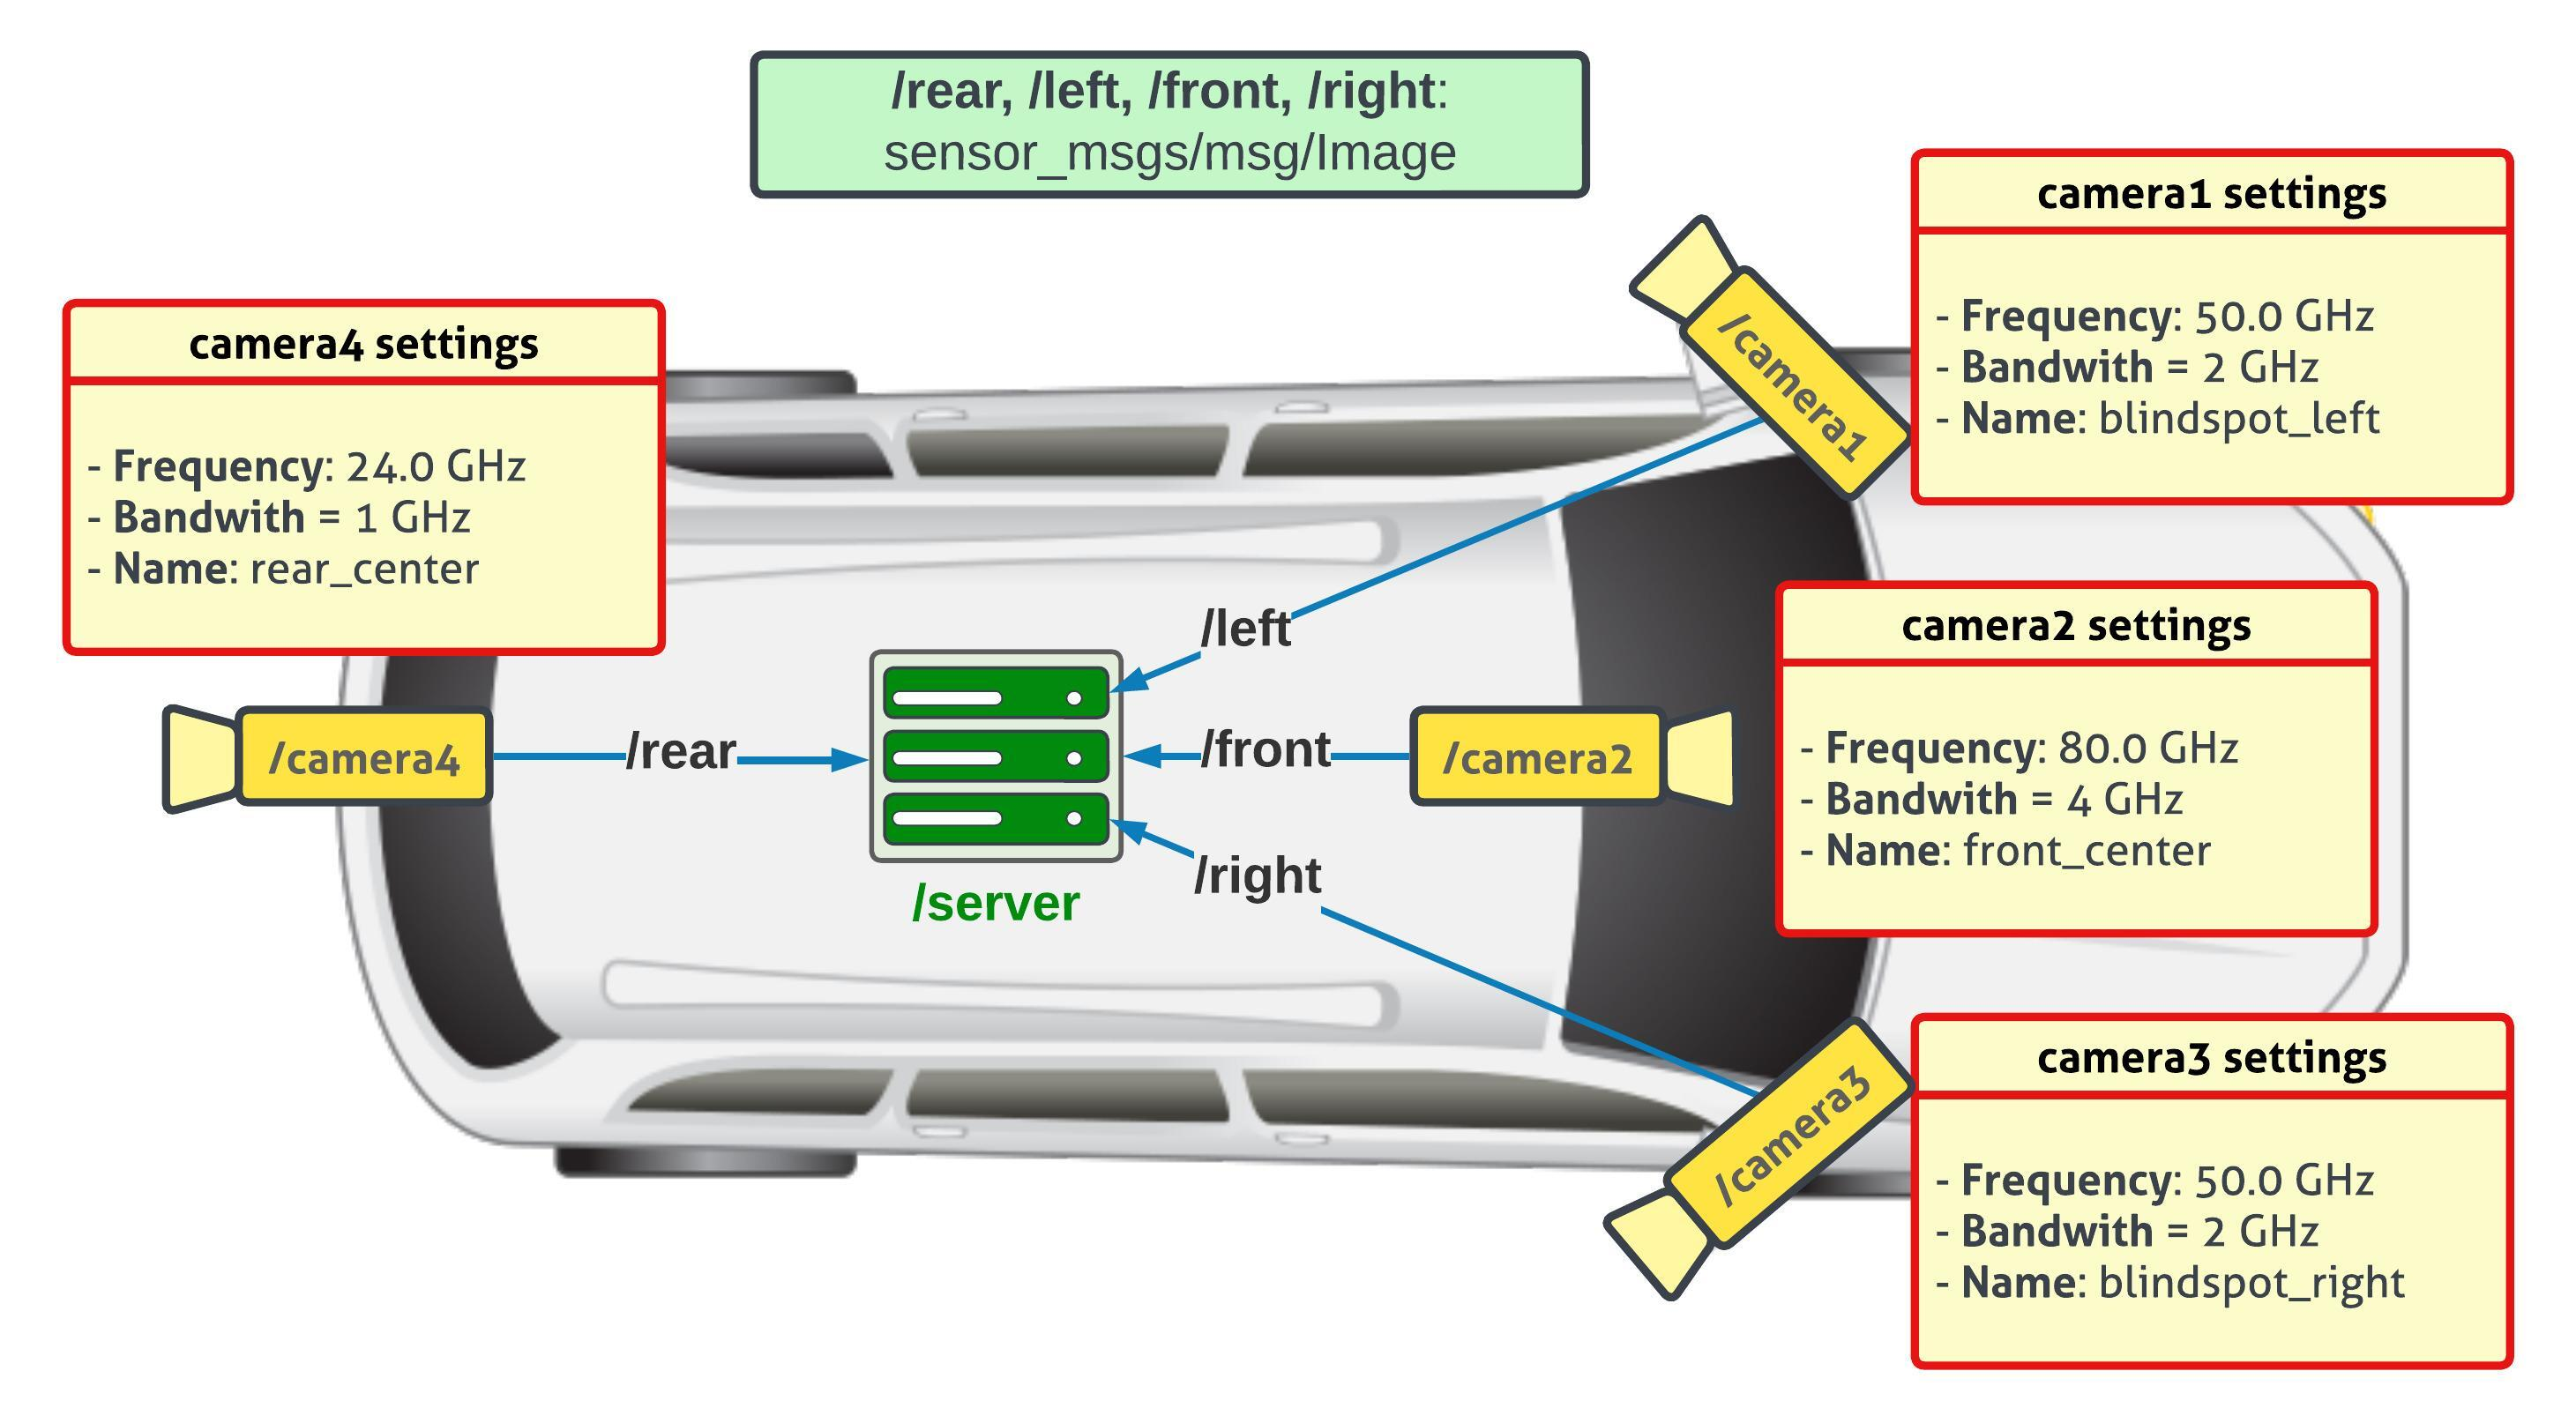
\includegraphics[width=10.5cm]{figures/lecture5/av.jpeg}
\end{figure}
\end{center}

\vspace*{\fill}
\end{frame}
%#####################################


\subsection{CLI}
%#####################################
\begin{frame}[fragile]{\secsec}
\vspace*{\fill}

{\mynote CLI for Parameters} \doublerulefill

\begin{center}
\begin{compactitem}
    \item \myTerminal{ros2 param -h}
\begin{textscript}
usage: ros2 param [-h] Call `ros2 param <command> -h` for more detailed usage. ...

Various param related sub-commands

optional arguments:
  -h, --help            show this help message and exit

Commands:
  delete    Delete parameter
  describe  Show descriptive information about declared parameters
  dump      Dump the parameters of a node to a yaml file
  get       Get parameter
  list      Output a list of available parameters
  load      Load parameter file for a node
  set       Set parameter

  Call `ros2 param <command> -h` for more detailed usage.
\end{textscript}
\end{compactitem}
\end{center}

\vspace*{\fill}
\end{frame}
%#####################################

%#####################################
% \begin{frame}[fragile]{\sec}
% \vspace*{\fill}

% {\myNote CLI Usage Examples for Parameters} \doublerulefill

% \begin{center}
% \begin{compactitem}
% \small
%     \item \myTerminal{ros2 launch first_package first_package_1.launch.py}
%     \item \myTerminal{ros2 param list}
%     \item Get the value of a Parameter for a running Node: \myTerminalBlank{ros2 param get <node> <parameter>}
%     \begin{compactitem}
%         \item \myTerminal{ros2 param get /advanced_publisher use_sim_time}
%         \begin{textscript}
% Boolean value is: False
% \end{textscript}
%     \end{compactitem}
%     \item Set the value of a Parameter for a running Node: \myTerminalBlank{ros2 param set <node> <parameter> <value>}
%     \begin{compactitem}
%         \item \myTerminal{ros2 param set /advanced_publisher jedi 'Luke Skywalker'}
%         \begin{textscript}
% Setting parameter failed: ('Invalid access to undeclared parameter(s)', [])
% \end{textscript}
% \end{compactitem}
% \end{compactitem}
% \end{center}

% \vspace*{\fill}
% \end{frame}
%#####################################


\subsection{Programming}
%#####################################
\begin{frame}[fragile]{\secsec}
\vspace*{\fill}

{\mynote Programming} \doublerulefill

\begin{center}
\emph{Parameters should be declared before their uses.}

\hrulefill


\begin{compactenum}
\small
    \item Declare the Parameter.
    
    \begin{compactitem}
        \footnotesize
        \item \mybestpractice Give a default value when declaring a Parameter. The default value can be overwritten at run time.
        \item[] \raisebox{\dimexpr-\height+7pt}{
\includegraphics[height=10pt, width=10pt]{figures/icons/cpp.png}}  \mscript{this->declare_parameter("jedi", "Obi-Wan Kenobi");}
        \item[] \faIcon{python}  \pscript{self.declare_parameter('jedi', 'Obi-Wan Kenobi')}
    \end{compactitem}
    \item Retrieve the Parameter.
\begin{compactitem}
\footnotesize
\item[] \raisebox{\dimexpr-\height+7pt}{
\includegraphics[height=10pt, width=10pt]{figures/icons/cpp.png}} \mscript{jedi_ = this->get_parameter("jedi").as_string();}
\item[] \faIcon{python} \pscript{self._jedi = self.get_parameter('jedi').get_parameter_value().string_value}
\end{compactitem}
    \item Use the Parameter.
\begin{compactitem}
\item After storing the Parameter value in an attribute, use the attribute in your code.
\begin{compactitem}
\footnotesize
\item[] \raisebox{\dimexpr-\height+7pt}{
\includegraphics[height=10pt, width=10pt]{figures/icons/cpp.png}} \mscript{msg_.data = "Help me " + jedi_ + ", you are my only hope.";}
\item[] \faIcon{python} \pscript{self._msg.data = f'Help me {self._jedi}, you are my only hope.'}
\end{compactitem}
\end{compactitem}
\end{compactenum}
\end{center}

\vspace*{\fill}
\end{frame}
%#####################################

\subsection{Set Parameters}
\subsubsection*{Command Line}
%#####################################
\begin{frame}[fragile]{\secsecsec}
\vspace*{\fill}

{\mynote Set Parameter on the Command Line} \doublerulefill

\begin{center}
\emph{You can start a Node and at the same time set  Parameter values. If a value is not provided on the command line, the default one from the code will be used.}

\hrulefill


\begin{compactitem}
\small
\item \myTerminalBlank{-{}-ros-args} to pass arguments to a Node on the command line.
\item \myTerminalBlank{-p <parameter>:=<value>} to set a value for a Parameter.
\item \myTerminal{ros2 run parameter_demo parameter_demo_exe}
\begin{textscript}
[INFO] [...] [parameter_demo]: Help me Obi-Wan Kenobi, you are my only hope.
\end{textscript}

\item \myTerminal{ros2 run parameter_demo parameter_demo_exe -{}-ros-args -p jedi:=\textquotesingle Luke Skywalker\textquotesingle}

\begin{textscript}
[INFO] [...] [parameter_demo]: Help me Luke Skywalker, you are my only hope.
\end{textscript}

\end{compactitem}
\end{center}

\vspace*{\fill}
\end{frame}
%#####################################

% \subsection{Pass to Launch File}

% \subsubsection*{Python}
\subsubsection*{Launch File}
%#####################################
\begin{frame}[fragile]{\secsecsec}
\vspace*{\fill}

{\mynote Set Parameters in Launch Files} \doublerulefill

\begin{center}
\begin{compactitem}
\small
\begin{pyscript}
import os
from launch import LaunchDescription
from launch_ros.actions import Node
from ament_index_python.packages import get_package_share_directory

def generate_launch_description():
    
    parameter_individual_demo = Node(
        package="parameter_demo",
        executable="parameter_demo_exe.py",
        parameters=[
            {'jedi': 'Luke Skywalker'},
        ],
    )
    
    ld = LaunchDescription()
    ld.add_action(parameter_individual_demo)   
    return ld  
\end{pyscript}

\item \myTerminal{ros2 launch parameter_demo parameter_demo.launch.py}
\end{compactitem}
\end{center}

\vspace*{\fill}
\end{frame}
%#####################################

\subsection{Multiple Parameters}
%#####################################
\begin{frame}[fragile]{\secsec}
\vspace*{\fill}

{\mynote Parameter Files} \doublerulefill

\begin{center}
\emph{Managing Parameters can become a real problem if your Node has many Parameters. There are multiple ways to provide multiple Parameters for a Node.}
\end{center}


\begin{compactenum}
\footnotesize

\item Passing multiple parameters to the command line.
\begin{compactitem}
    \footnotesize
    \item \myTerminal{ros2 run <package> <exe> -{}-ros-args -p <param>:=<value> -p <param>:=<value> ...}
\end{compactitem}

\item Passing multiple individual Parameters to the launch file.
\begin{pyscriptII}
parameter_individual_demo = Node(
    package="<package>",
    executable="<executable>",
    parameters=[
        {"<param>": <value>},
        {"<param>": <value>},
        {"<param>": <value>},
        ...
    ],
)
\end{pyscriptII}
\item Passing a Parameter file to the command line.
\item Passing a Parameter file to the launch file.
\end{compactenum}

% \begin{center}
% \emph{Managing Parameters can become a real problem if your Node has many Parameters.}
% \begin{compactitem}
% \small
% \item Adding Parameters from command line can be very tedious.
% \item  You can add each one of them in a launch file, but that will also take many lines in your launch file, and for each different configuration you will have to write different launch files.
% \item You can set all your Parameters in a YAML file and then load this YAML file for your Node.
% \end{compactitem}
% \end{center}

\vspace*{\fill}
\end{frame}
%#####################################

%#####################################
\subsubsection*{Parameter File}
\begin{frame}[fragile]{\secsecsec}
\vspace*{\fill}
\begin{center} 

{\mytodo Set Parameters in a YAML File} \doublerulefill


\begin{compactitem}
\footnotesize
    \item Create the folder \myFolder{config} in the package (you can use an arbitrary name).
    \item Create the file \myFile{params.yaml} in \myFolder{config} (you can use an arbitrary name).
    \item Add the following in \myFile{params.yaml}
\begin{yamlscriptII}
parameter_demo_node:  # Name of your Node
  ros__parameters:
    jedi: 'Luke Skywalker'
\end{yamlscriptII}
\end{compactitem}

{\mytodo Edit \myFile{CMakeLists.txt}} \doublerulefill


\begin{compactitem}
\footnotesize
    \item You need to install the \myFolder{config}.
    \begin{compactitem}
    \footnotesize
    \item In \myFile{CMakeLists.txt}, mark the folder \myFolder{config} for installation.
    \begin{cmakescript}
install(DIRECTORY
  include
  launch
  config
  DESTINATION share/${PROJECT_NAME}
)
    \end{cmakescript}
    \end{compactitem}
\end{compactitem}

{\mytodo Build your Package} \doublerulefill

\begin{compactitem}
\footnotesize
    \item \myTerminal{colcon build}
\end{compactitem}


\end{center}
\vspace*{\fill}
\end{frame}


% \subsubsection*{Command Line}
%#####################################
\begin{frame}[fragile]{\secsecsec}
\vspace*{\fill}

{\mynote Use the Parameter File on the Command Line} \doublerulefill



\begin{center}
\emph{Use the Parameter file on the command line by providing the path to the file (relative or absolute).}

\hrulefill

\begin{compactitem}
\footnotesize

\item[] \myTerminal{ros2 run parameter_demo parameter_demo_exe -{}-ros-args -{}-params-file <path to parameter file>}
\end{compactitem}
\end{center}
\vspace*{\fill}
\end{frame}
%#####################################


\subsubsection*{Launch File}
%#####################################
\begin{frame}[fragile]{\secsec}
\vspace*{\fill}

{\mynote Use the Parameter File in the Launch File} \doublerulefill


\begin{compactitem}
\footnotesize
\item Get the path to the Parameter file.
\begin{pyscriptII}
import os
from ament_index_python.packages import get_package_share_directory
\end{pyscriptII}

\begin{pyscriptII}
node_params = os.path.join(
        get_package_share_directory('parameter_demo'),
        'config',
        'params.yaml'
)
\end{pyscriptII}

\item[] or

\begin{pyscriptII}
from launch.substitutions import PathJoinSubstitution
from launch_ros.substitutions import FindPackageShare
\end{pyscriptII}

\begin{pyscriptII}
node_params = PathJoinSubstitution(
        [FindPackageShare("parameter_demo"), "config", "params.yaml"]
)
\end{pyscriptII}
\item Pass the Parameter file to the Node.
\begin{pyscriptII}
parameter_file_demo = Node(
        package="parameter_demo",
        executable="parameter_demo_exe.py",
        parameters=[node_params],
    )
\end{pyscriptII}
\end{compactitem}
\vspace*{\fill}
\end{frame}
%#####################################


\subsection{Modify Parameters}
%#####################################
\begin{frame}[fragile]{\secsec}
\vspace*{\fill}

{\mynote Modify a Parameter at Runtime} \doublerulefill

\begin{center}
\begin{compactitem}
\small
\item \myTerminal{ros2 run parameter_demo parameter_demo_exe}
\item \myTerminal{ros2 param set /parameter_demo_node jedi \textquotesingle Luke Skywalker\textquotesingle}
\begin{textfoot}
Set parameter successful
\end{textfoot}
\item \myTerminal{ros2 param get /parameter_demo_node jedi}
\begin{textfoot}
String value is: Luke skywalker
\end{textfoot}
\item The value of \myParameter{jedi} has changed, but in the code, the attribute value  is still the old one! If you change a Parameter's value after it has been read by the Node, then the Node will not be able to know it, unless you notify the Node about the change. 
\begin{compactitem}
    \item We need to add a callback to notify the Node as soon as the Parameter has been modified.
\end{compactitem}
\end{compactitem}
\end{center}

\vspace*{\fill}
\end{frame}
%#####################################


\subsubsection*{Callback}

% \subsubsection*{Python}
%#####################################
\begin{frame}[fragile]{\secsecsec}
\vspace*{\fill}

{\faIcon{python} Callback for Parameter Changes} \doublerulefill

\begin{center}
\begin{compactitem}
\small
\begin{pyscriptII}
from rclpy.parameter import Parameter
from rcl_interfaces.msg import SetParametersResult

class ParameterDemoNode(Node):

  def __init__(self, node_name):
    # Callback for parameter changes
    self.add_on_set_parameters_callback(self.parameters_callback)
    ...

  def parameters_callback(self, params):
        success = False
        for param in params:
            if param.name == "jedi":
                if param.type_ == Parameter.Type.STRING:
                    success = True
                    self._jedi = param.value # modify the attribute
        return SetParametersResult(successful=success)
\end{pyscriptII}
\end{compactitem}
\end{center}

\vspace*{\fill}
\end{frame}
%#####################################

% \subsubsection*{\CC}
%#####################################
\begin{frame}[fragile]{\secsecsec}
\vspace*{\fill}

{\raisebox{\dimexpr-\height+8pt}{
\includegraphics[height=10pt, width=10pt]{figures/icons/cpp.png}} Callback for Parameter Changes} \doublerulefill

\begin{center}
\begin{compactitem}
\small
\begin{cppscriptII}
// parameter_demo.hpp
#include "rcl_interfaces/msg/set_parameters_result.hpp"

class ParameterDemoNode : public rclcpp::Node
{
public:
    ParameterDemoNode(std::string node_name) : Node(node_name)
    {
        // callback for parameter change
        callback_handle_ = this->add_on_set_parameters_callback(
            std::bind(&ParameterDemoNode::parametersCallback, this, std::placeholders::_1));
        ...
    }

private:
    // attributes
    OnSetParametersCallbackHandle::SharedPtr callback_handle_;

    // methods
    rcl_interfaces::msg::SetParametersResult parametersCallback(
      const std::vector<rclcpp::Parameter> &parameters
    );
};
\end{cppscriptII}
\end{compactitem}
\end{center}

\vspace*{\fill}
\end{frame}
%#####################################



%#####################################
\begin{frame}[fragile]{\secsecsec}
\vspace*{\fill}

{\raisebox{\dimexpr-\height+8pt}{
\includegraphics[height=10pt, width=10pt]{figures/icons/cpp.png}}  Callback for Parameter Changes} \doublerulefill

\begin{center}
\begin{compactitem}
\small
\begin{cppscriptII}
// parameter_demo.cpp
rcl_interfaces::msg::SetParametersResult ParameterDemoNode::parametersCallback(
    const std::vector<rclcpp::Parameter> &parameters)
{
    rcl_interfaces::msg::SetParametersResult result;
    result.successful = true;
    result.reason = "success";
    for (const auto &param : parameters)
    {
        if (param.get_name() == "jedi")
        {
            jedi_ = param.as_string(); // modify the attribute
        }
        else
        {
            result.successful = false;
            result.reason = "parameter name not found";
        }
    }
    return result;
}
\end{cppscriptII}
\end{compactitem}
\end{center}

\vspace*{\fill}
\end{frame}
%#####################################




%#####################################
\section{Name Remapping}

%#####################################
\begin{frame}[fragile]{\sec}
\vspace*{\fill}

{\mydefinition Name Remapping } \doublerulefill

\begin{center}
\emph{Name remapping is a technique used to give Nodes and Topics a different name at runtime. With name remapping, multiple instances of Nodes and Topics are created to avoid code duplication.}
\end{center}

\vspace*{\fill}
\end{frame}



\subsection{Example}
%#####################################
\begin{frame}[fragile]{\secsec}
\vspace*{\fill}

\begin{figure}
    \centering
    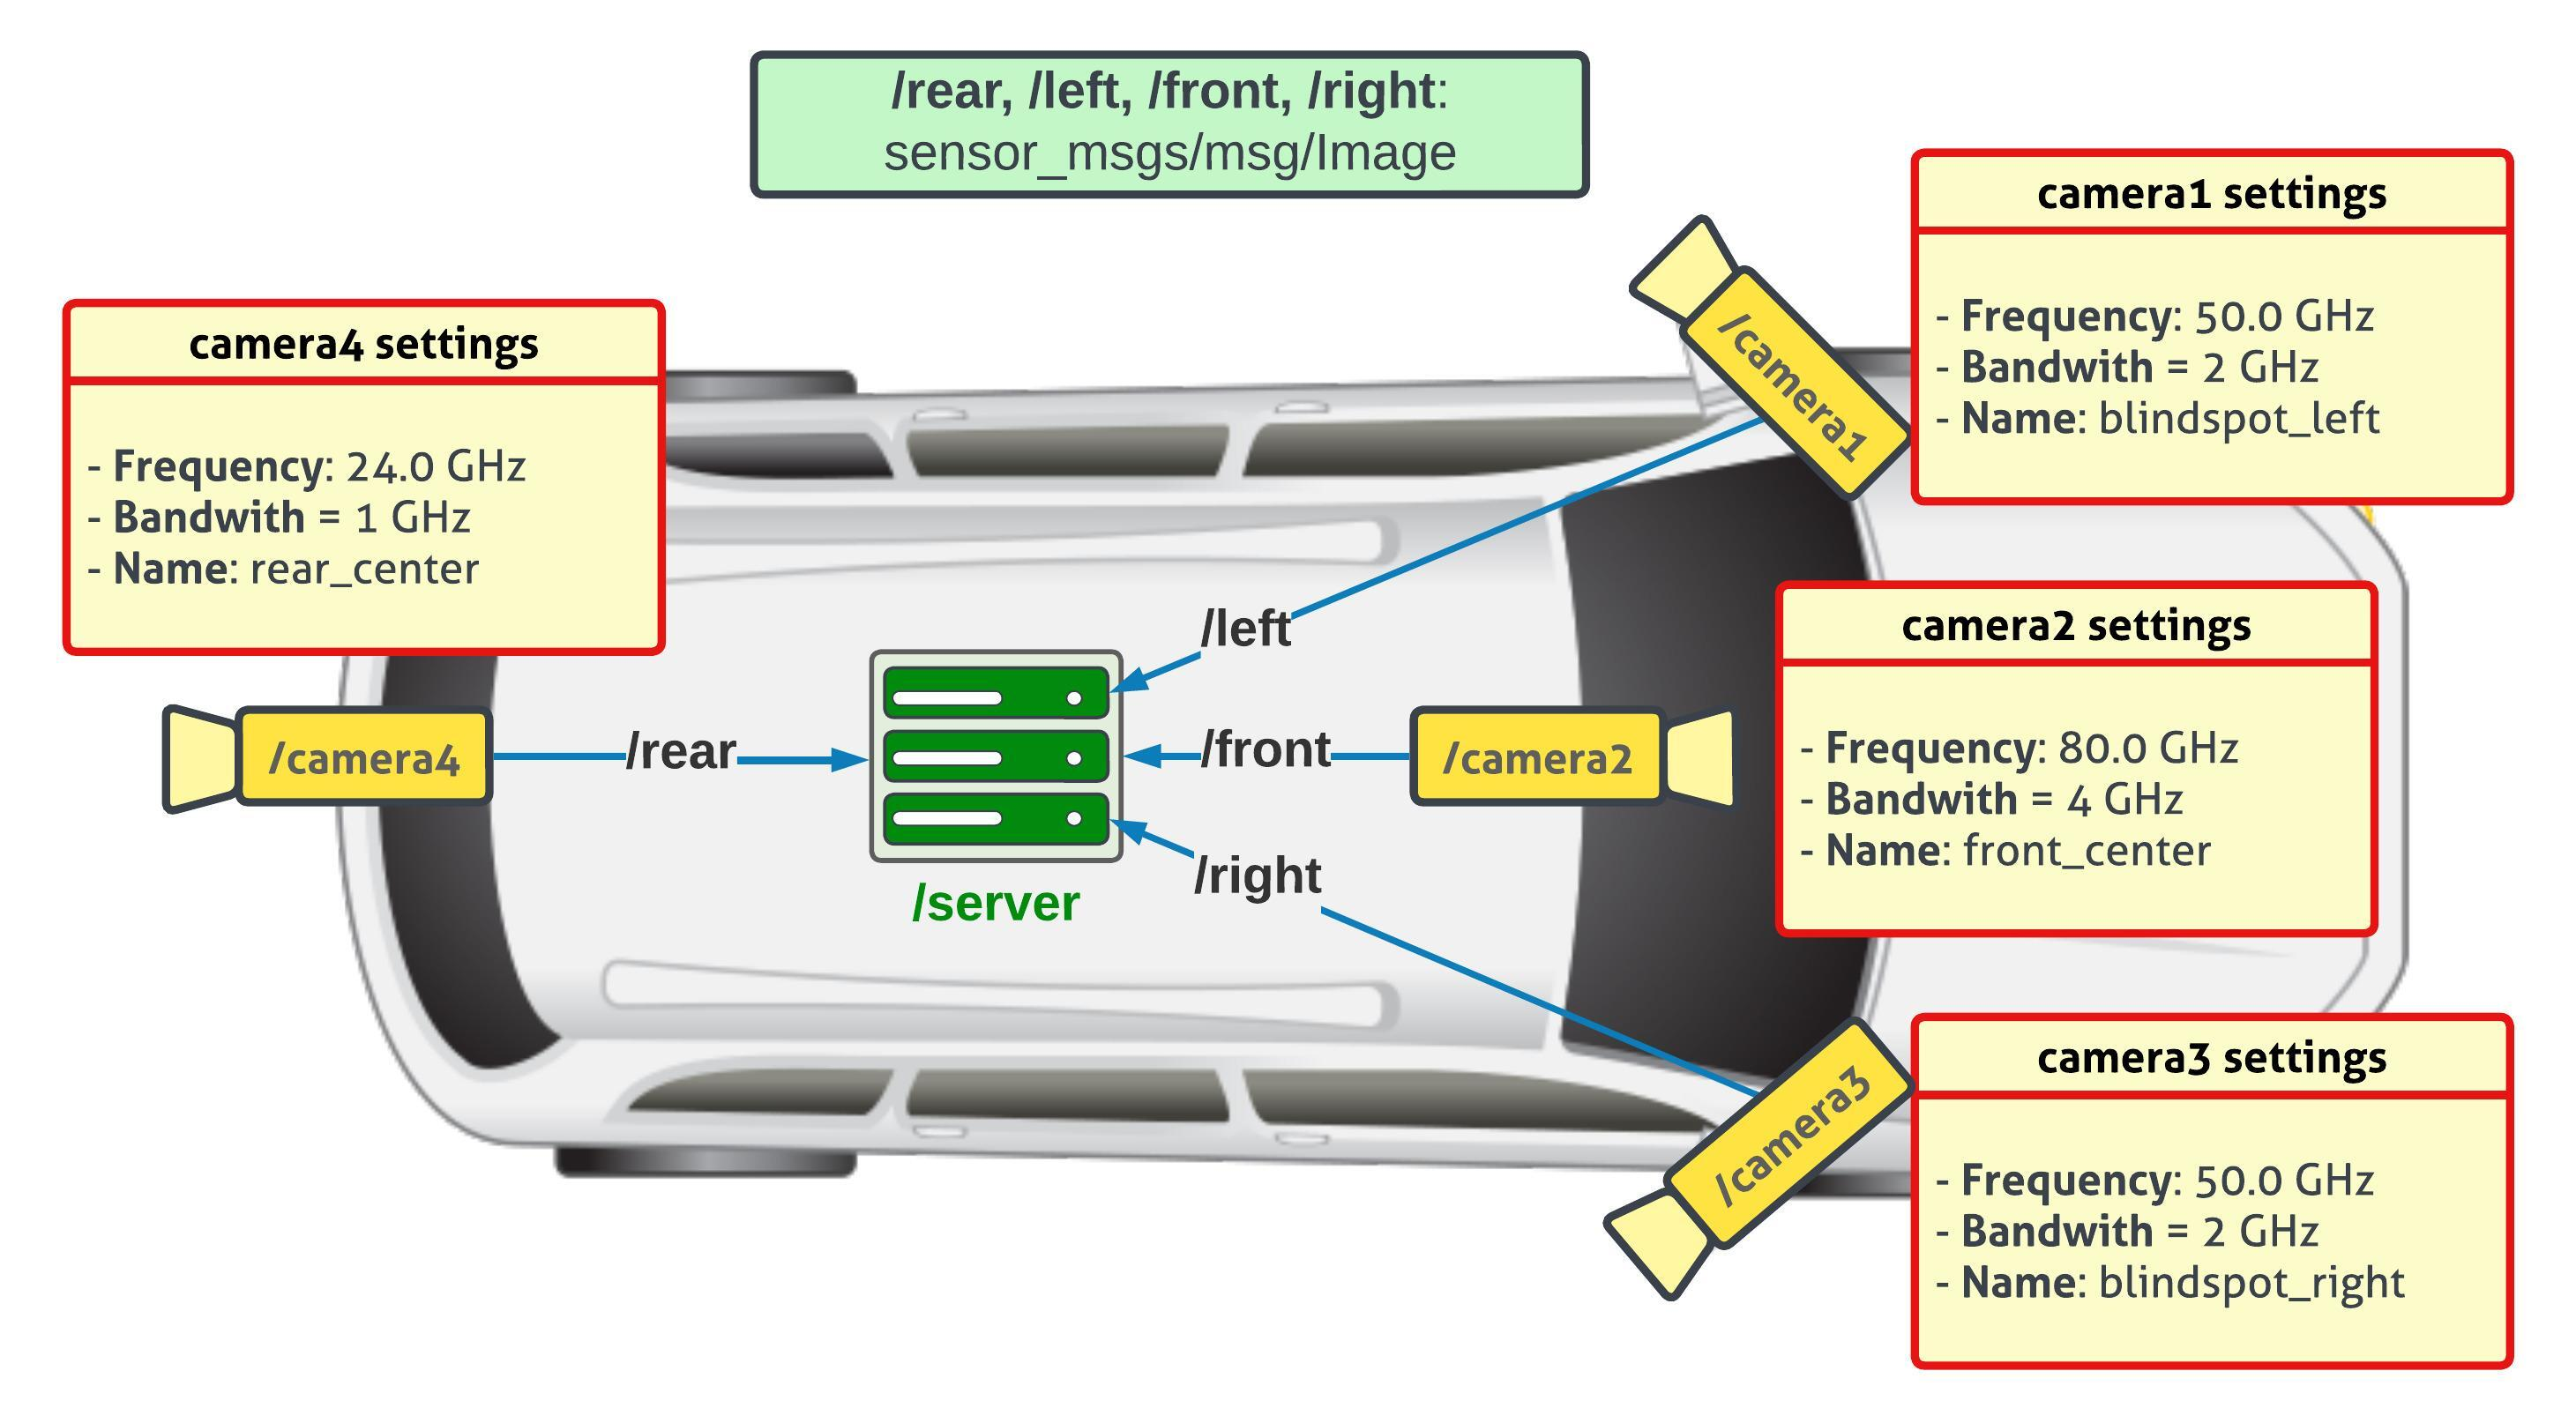
\includegraphics[width=10.5cm]{figures/lecture5/av.jpeg}
\end{figure}

\begin{compactitem}
    \small
    \item Each \myNode{/camera\{n\}} publishes \myMessage{sensor_msgs/msg/Image} to a Topic.
    \item \myNode{/server} is subscribed to each camera Topic.
\end{compactitem}
\vspace*{\fill}
\end{frame}


%#####################################
\begin{frame}[fragile]{\secsec}
\vspace*{\fill}
\begin{compactitem}
    \item Each camera does the exact same thing:
    \begin{compactenum}
    \item Retrieves information about the environment.
    \item Publishes this information to a Topic.
    \end{compactenum}

\item In this situation, you do not need to write four different \myNode{/camera} Nodes.
\item You can write one generic Node and execute it for each camera.
\begin{compactitem}
    \item You need to provide the correct Node name for your camera: \myNode{camera1}, \myNode{camera2}, \myNode{camera3}, or \myNode{camera4}
    \item You need to provide the correct Topic name for each Node: \myTopic{front}, \myTopic{left}, \myTopic{right}, or \myTopic{rear}
\end{compactitem}
\end{compactitem}
\vspace*{\fill}
\end{frame}

\subsection{Command Line}
\begin{frame}[fragile]{\secsec}
\vspace*{\fill}
\begin{center} 
%%%%%%%%%%%%%%%%%%%%%%%%%%%%%%%%%%%%%%%%%%%%%%%%

{\mydefinition Command Line Name Remapping } \doublerulefill


\emph{Name remapping on the command line is done with \myTerminalBlank{-{}-ros-args} and \myTerminalBlank{-{}-remap} (or \myTerminalBlank{-r})}

\hrulefill

\begin{compactitem}
    \item To remap a Node: \myTerminalBlank{_{}_node:=<new name>}
    \item To remap a Topic: \myTerminalBlank{<current name>:=<new name>}
    \item Example for camera1:
    \item[]\myTerminal{ros2 run automated_vehicle camera_exe.py -{}-ros-args -r _{}_node:=camera1 \backslash}
    \item[]~~~~~~\myTerminalBlank{> -r camera:=left -{}-params-file <path to parameter file>}
\end{compactitem}
\end{center}
\vspace*{\fill}
\end{frame}


\subsection{Launch File}
\begin{frame}[fragile]{\secsec}
\vspace*{\fill}
\begin{center} 
%%%%%%%%%%%%%%%%%%%%%%%%%%%%%%%%%%%%%%%%%%%%%%%%

{\mydefinition Name Remapping in Launch Files} \doublerulefill

\begin{compactitem}
    \item Example for camera1:
\begin{pyscript}
camera1_python = Node(
    package="automated_vehicle",
    executable="camera_exe.py",
    parameters=[node_params],   # parameter file
    name='camera1',             # node remapping
    remappings=[                # topic remapping   
        ('/camera', '/left')
    ],
    parameters=[node_params]    # parameter file if needed
)
\end{pyscript}
\end{compactitem}

\end{center}
\vspace*{\fill}
\end{frame}


%%%%%%%%%%%%%%%%%%
%#####################################
\section{Executor}
%#####################################
\begin{frame}[fragile]{\sec}
\vspace*{\fill}
{\mydefinition Executor}\doublerulefill


\emph{An \urllink{https://docs.ros.org/en/galactic/Concepts/About-Executors.html}{executor} controls the threading model used to process callbacks. Callbacks are units of work like subscription callbacks, timer callbacks, service calls, and received client responses. An executor controls which threads callbacks get executed in.}

\begin{compactitem}
    \small
    \item By default, \pscript{rclpy} offers two different executors and \mscript{rclcpp} offers three different executors.
    \begin{compactitem}
        \footnotesize
        \item \emph{SingleThreadedExecutor} (default) is quite straightforward: It executes callbacks in a single thread, one at a time, and thus the previous callback must always finish before a new one can begin execution.
        \item \emph{MultiThreadedExecutor} on the other hand, is capable of executing several callbacks simultaneously. 
        \item \urllink{https://docs.ros.org/en/ros2_packages/humble/api/rclcpp/generated/classrclcpp_1_1executors_1_1StaticSingleThreadedExecutor.html}{StaticSingleThreadedExecutor} (only in \CC) optimizes the runtime costs for scanning the structure of a node in terms of subscriptions, timers, service servers, action servers, etc. It performs this scan only once when the Node is added, while the other two executors regularly scan for such changes. Therefore, \emph{StaticSingleThreadedExecutor} should be used only with Nodes that create all subscriptions, timers, etc. during initialization.
    \end{compactitem}
\end{compactitem}
\vspace*{\fill}
\end{frame}


\subsection{Callback Groups}

\begin{frame}[fragile]{\secsec}
\vspace*{\fill}
{\mydefinition Callback Groups}\doublerulefill

\emph{SingleThreadedExecutor does not care about any callback group options. Thus we will not discuss it further, and the following topics only concern the MultiThreadedExecutor.}

\begin{compactitem}
    \footnotesize
    \item There two different callback groups to work in combination with \emph{MultiThreadedExecutors}:
    \begin{compactitem}
        \footnotesize
        \item \emph{MutuallyExclusiveCallbackGroup} allows the executor to execute only one of its callbacks at a time, essentially making it as if the callbacks in the group were executed by a \emph{SingleThreadedExecutor}. Thus, it is a good choice to put any callbacks accessing critical and potentially \emph{non-thread-safe resources} in the same \emph{MutuallyExclusiveCallbackGroup}.
        \item \emph{ReentrantCallbackGroup} allows the executor to schedule and execute the group's callbacks in any way the executor sees fit, without restrictions. In computing, a computer program or subroutine is called reentrant if multiple invocations can safely run concurrently on multiple processors, or on a single-processor system, where a reentrant procedure can be interrupted in the middle of its execution and then safely be called again (``re-entered") before its previous invocations complete execution.
    \end{compactitem}
\end{compactitem}
\vspace*{\fill}
\end{frame}


\begin{frame}[fragile]{\secsec}
\vspace*{\fill}
{\mydefinition Callback Groups}\doublerulefill


\begin{compactitem}
    \footnotesize
    \item In order to control execution with callback groups, one can consider the following guidelines (not an exhaustive list!).
    \begin{compactitem}
        \footnotesize
        \item Register callbacks accessing critical non-thread-safe resources in the same \inpy{MutuallyExclusiveCallbackGroup} (or protect the resources by locks manually).
        \item If you have a callback whose execution instances need to be able to overlap with each other, register it to a \emph{ReentrantCallbackGroup}.
        \item If you have callbacks that require to be potentially executed in parallel to one another, register them to:
        \begin{compactitem}
            \footnotesize
            \item A \emph{ReentrantCallbackGroup}, or
            \item Different \emph{MutuallyExclusiveCallbackGroups} (this option is good if you want the callbacks to not overlap themselves, or also need or want thread safety with respect to some other callbacks).
            \begin{compactitem}
                \footnotesize
                \item This is a valid way of allowing parallel execution for different callbacks, and can even be more desirable than simply registering everything into one \emph{ReentrantCallbackGroup}.
            \end{compactitem}
        \end{compactitem}
    \end{compactitem}
\end{compactitem}
\vspace*{\fill}
\end{frame}



%#####################################
\section{Interfaces}
%#####################################
\begin{frame}[fragile]{\sec}
\vspace*{\fill}
\begin{center} 
{\mydefinition Interfaces} \doublerulefill

\emph{ROS applications typically communicate through \urllink{https://docs.ros.org/en/foxy/Concepts/About-ROS-Interfaces.html}{interfaces} of one of three types: Messages, Services, and Actions.}

\hrulefill

\emph{ROS2 uses the interface definition language (IDL) to describe these interfaces. This description makes it easy for ROS tools to automatically generate source code for the interface type in several target languages.}

\hrulefill

\begin{compactitem}
\small
    \item \myTerminal{ros2 interface list} lists all the interfaces installed on your system. These interfaces are defined in static files which are then used to generate \CC and Python classes with \myTerminal{colcon build}
    \item To create custom interfaces, it is highly recommended to create a package only for custom interfaces.
    \begin{compactitem}
        \item \mynote This package does not contain any code.
    \end{compactitem}
\end{compactitem}

\end{center}
\vspace*{\fill}
\end{frame}


%%%%%%%%%%%%%%%%%%%%%%%%%%%%%%%%%%%
\begin{frame}[fragile]{\sec}
\vspace*{\fill}
\begin{center} 

{\mytodo Create a \CC package for Interfaces} \doublerulefill

\begin{compactitem}
    \item Create the \CC package \myROSPackage{enpm663_msgs}
    \begin{compactitem}
        \item \myTerminal{ros2 pkg create enpm663_msgs -{}-dependencies std_msgs builtin_interfaces}
        \item You can delete \myFolder{src} and \myFolder{include} since we will not write any code in this package.
    \end{compactitem}
    \item In the package, create 2 folders: \myFolder{msg} and \myFolder{srv}
    \begin{compactitem}
        \item Create \myFile{WeatherStation.msg}  in \myFolder{msg} 
        \begin{compactitem}
            \item This Message provides information on the current weather.
        \end{compactitem}
        \item Create \myFile{AddTwoInts.srv}  in \myFolder{srv} 
        \begin{compactitem}
            \item This Service will take two integers, add them together, and return the result.
        \end{compactitem}
    \end{compactitem}
\end{compactitem}

{\mywarning} \doublerulefill

It is important that these files use CamelCase naming convention (the first letter of each word is uppercase and underscores are not used.

\end{center}
\vspace*{\fill}
\end{frame}



%%%%%%%%%%%%%%%%%%%%%%%%%%%%%%%%
\begin{frame}[fragile]{\sec}
\vspace*{\fill}
\begin{center} 

{\mytodo Define Messages and Services} \doublerulefill


\begin{columns}
    \column{0.5\textwidth}
        \centering
\begin{compactitem}
    \item In \myFile{WeatherStation.msg}
    \begin{textfoot}
|\textcolor{RedOrange}{uint8}| |\textcolor{RoyalBlue}{CLOUDY}|=0
|\textcolor{RedOrange}{uint8}| |\textcolor{RoyalBlue}{SUNNY}|=1
|\textcolor{RedOrange}{uint8}| |\textcolor{RoyalBlue}{SNOWY}|=2


|\textcolor{RedOrange}{uint8}| weather
|\textcolor{RedOrange}{uint8}| day
|\textcolor{RedOrange}{builtin\_interfaces/Time}| time
    \end{textfoot}
    
\end{compactitem}
    \column{0.5\textwidth}
\begin{compactitem}
    \item In \myFile{AddTwoInts.srv}
    \begin{textfoot}
|\textcolor{RedOrange}{int64}| a
|\textcolor{RedOrange}{int64}| b
---
|\textcolor{RedOrange}{int64}| sum
    \end{textfoot}
    
\end{compactitem}
\end{columns}

\end{center}
\vspace*{\fill}
\end{frame}


\subsubsection*{Generation}
%%%%%%%%%%%%%%%%%%%%%%%%%%%%%%%%%%%
\subsection{Message}
%%%%%%%%%%%%%%%%%%%%%%%%%%%%%%%%%%%

\begin{frame}[fragile]{\secsec}
\vspace*{\fill}
\begin{center} 
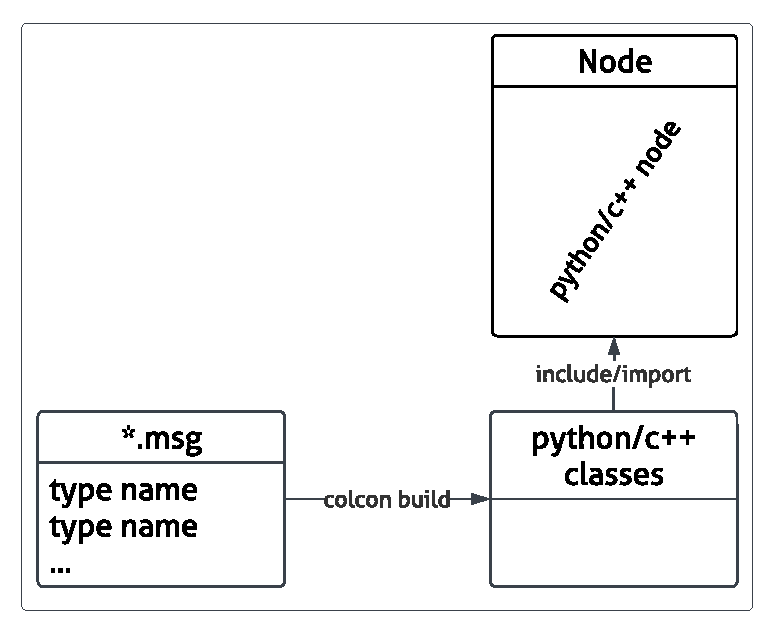
\includegraphics[width=10cm]{figures/lecture5/msg.pdf}
\end{center}
\vspace*{\fill}
\end{frame}



\begin{frame}[fragile]{\secsecsec}
\vspace*{\fill}
\begin{center} 
{\mytodo Message Generation} \doublerulefill

\begin{compactitem}

\item \urllink{https://docs.ros.org/en/galactic/Tutorials/Beginner-Client-Libraries/Single-Package-Define-And-Use-Interface.html#build-a-msg-file}{Build a msg file}: Add the following in \myFile{package.xml}

\begin{xmlscript}
<buildtool_depend>rosidl_default_generators</buildtool_depend>
<exec_depend>rosidl_default_runtime</exec_depend>
<depend>builtin_interfaces</depend>
<depend>std_msgs</depend>  

<member_of_group>rosidl_interface_packages</member_of_group>
\end{xmlscript} 

\end{compactitem}
\end{center}
\vspace*{\fill}
\end{frame}



%%%%%%%%%%%%%%%%%%%%%%%%%%%%%%%%%%%
\begin{frame}[fragile]{\secsecsec}
\vspace*{\fill}
\begin{center} 
{\mytodo Message Generation} \doublerulefill

\begin{compactitem}

\item \urllink{https://docs.ros.org/en/galactic/Tutorials/Beginner-Client-Libraries/Single-Package-Define-And-Use-Interface.html#build-a-msg-file}{Build a msg file}: Add the following in \myFile{CMakeLists.txt}

\begin{cmakescript}
# find dependencies
find_package(ament_cmake REQUIRED)
find_package(std_msgs REQUIRED)
find_package(builtin_interfaces REQUIRED)
find_package(rosidl_default_generators REQUIRED)

set(msg_files
  "msg/WeatherStation.msg"
)

rosidl_generate_interfaces(${PROJECT_NAME}
  ${msg_files}

  DEPENDENCIES
  builtin_interfaces
  std_msgs
)

ament_export_dependencies(rosidl_default_runtime)
ament_package()
\end{cmakescript} 
\end{compactitem}
\end{center}
\vspace*{\fill}
\end{frame}

%#####################################
\begin{frame}[fragile]{\secsecsec}
\vspace*{\fill}
\begin{center} 
{\mytodo Generate Code for the Message} \doublerulefill

\begin{compactenum}
    \item Generate programming classes/struct for the Message:
    \begin{compactitem}
        \item \myTerminal{colcon build -{}-packages-select enpm663_msgs}
        \item \mywarning \myTerminal{source install/setup.bash}
        % \item \mywarning Source \myFile{setup.bash} of your workspace.
    \end{compactitem}
    \item Check related code has been generated in \myFolder{install}
    \item Check the custom Message can be found:
    \begin{compactitem}
        \item \myTerminal{ros2 interface show enpm663_msgs/msg/WeatherStation}
        \end{compactitem}
\end{compactenum}
\end{center}
\vspace*{\fill}
\end{frame}


\subsubsection*{Use}
%#####################################
\begin{frame}[fragile]{\secsecsec}
\vspace*{\fill}
\begin{center} 
{\mytodo Use the Message} \doublerulefill

\begin{compactenum}
\footnotesize
    \item \CC and Python classes were generated from the \myFile{WeatherStation.msg}
    \item To be able to use this Message in your code you need to:
    \begin{compactitem}
        \item Add the package \myROSPackage{enpm663_msgs} as a dependency.
        \item Include/import header file/module in your code.
    \end{compactitem}
\end{compactenum}

{\small \faIcon{python}} \doublerulefill

\begin{pyscript}
from enpm663_msgs.msg import WeatherStation
\end{pyscript}

{\raisebox{\dimexpr-\height+8pt}{
\includegraphics[height=10pt, width=10pt]{figures/icons/cpp.png}}} \doublerulefill

\begin{cppscriptII}
#include "enpm663_msgs/msg/weather_station.hpp"
\end{cppscriptII}

\begin{cmakescript}
find_package(rclcpp REQUIRED)
find_package(enpm663_msgs REQUIRED)
find_package(builtin_interfaces REQUIRED)

add_executable(message_demo_exe src/message_demo.cpp)
ament_target_dependencies(message_demo_exe rclcpp enpm663_msgs builtin_interfaces)
\end{cmakescript}

\begin{xmlscriptII}
<depend>enpm663_msgs</depend>
<depend>builtin_interfaces</depend>
<depend>rclcpp</depend>
\end{xmlscriptII}

\end{center}
\vspace*{\fill}
\end{frame}


%#####################################
\begin{frame}[fragile]{\secsecsec}
\vspace*{\fill}
\begin{center} 

{\mytodo Publish Custom Messages} \doublerulefill

\vspace{10pt}
\begin{compactitem}
\small
    
    \begin{tabular}{ l l}
    \footnotesize
    {\footnotesize Package} & \myROSPackage{interface_demo} \\
    {\footnotesize Files \raisebox{\dimexpr-\height+8pt}{
\includegraphics[height=9pt, width=9pt]{figures/icons/cpp.png}}} & \myFile{message_demo.cpp} and \myFile{message_demo.hpp} \\
    {\footnotesize Files \faIcon{python}} & \myFile{interface_demo.py} \\
    {\footnotesize Node} & \myNode{weather_forecast} \\
    {\footnotesize Topic} & \myTopic{weather} \\
    {\footnotesize Message} & \myMessage{enpm663_msgs/msg/WeatherStation} \\
    {\footnotesize Executable \raisebox{\dimexpr-\height+8pt}{
\includegraphics[height=9pt, width=9pt]{figures/icons/cpp.png}}} & \myExe{message_demo_exe}\\
    {\footnotesize Executable \faIcon{python}} & \myExe{message_demo_exe.py} \\
    \end{tabular} 

\item \faIcon{python} \myTerminal{ros2 run interface_demo message_demo_exe.py}
\item \raisebox{\dimexpr-\height+9pt}{
\includegraphics[height=10pt, width=10pt]{figures/icons/cpp.png}} \myTerminal{ros2 run interface_demo message_demo_exe}
\end{compactitem}

\end{center}
\vspace*{\fill}
\end{frame}

%#####################################
\subsection{Service}
%#####################################

\begin{frame}[fragile]{\secsec}
\vspace*{\fill}
\begin{center} 

{\mydefinition Services } \doublerulefill

\emph{\urllink{https://docs.ros.org/en/foxy/Tutorials/Beginner-CLI-Tools/Understanding-ROS2-Services/Understanding-ROS2-Services.html}{Services} are based on a call-and-response model. While Topics allow nodes to subscribe to data streams and get continual updates, Services only provide data when they are specifically called by a client (prevent unnecessary bandwidth usage).}

\begin{compactitem}
\small
    \item Use cases for Services:
    \begin{compactitem}
    \footnotesize
        \item Open/close gripper.
        \item Check an object is attached to a gripper.
        \item Query a sensor from time to time.
        \item Routine check for your robot.
    \end{compactitem}
    \item \mynote Only one server must be running and multiple clients can connect to the server.
    \item \mynote ROS2 allows for synchronous or asynchronous service calls.
    \begin{compactitem}
        \item \raisebox{\dimexpr-\height+8pt}{
\includegraphics[height=9pt, width=9pt]{figures/icons/cpp.png}} -- Asynchronous calls only.
        \item \faIcon{python} -- Asynchronous or synchronous calls.
    \end{compactitem}
\end{compactitem}
\end{center}
\vspace*{\fill}
\end{frame}


\begin{frame}[fragile]{\secsec}
\vspace*{\fill}
\begin{center} 
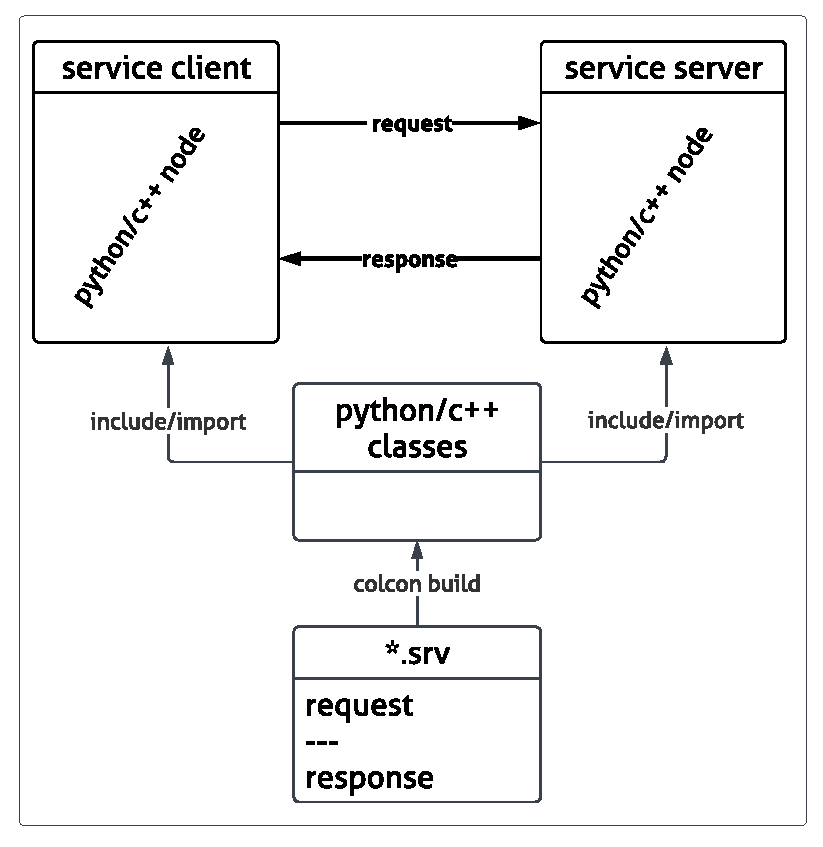
\includegraphics[width=8cm]{figures/lecture5/service.pdf}
\end{center}
\vspace*{\fill}
\end{frame}


%=+=+=+=+=+=+=+=+=+=+=+=+=+=+=+=+=+=+=+=+=+=+=+=+=+=
% \subsubsection*{Asynchronous Call}
% \begin{frame}[fragile]{\secsec}
% \vspace*{\fill}
% \begin{center} 
% 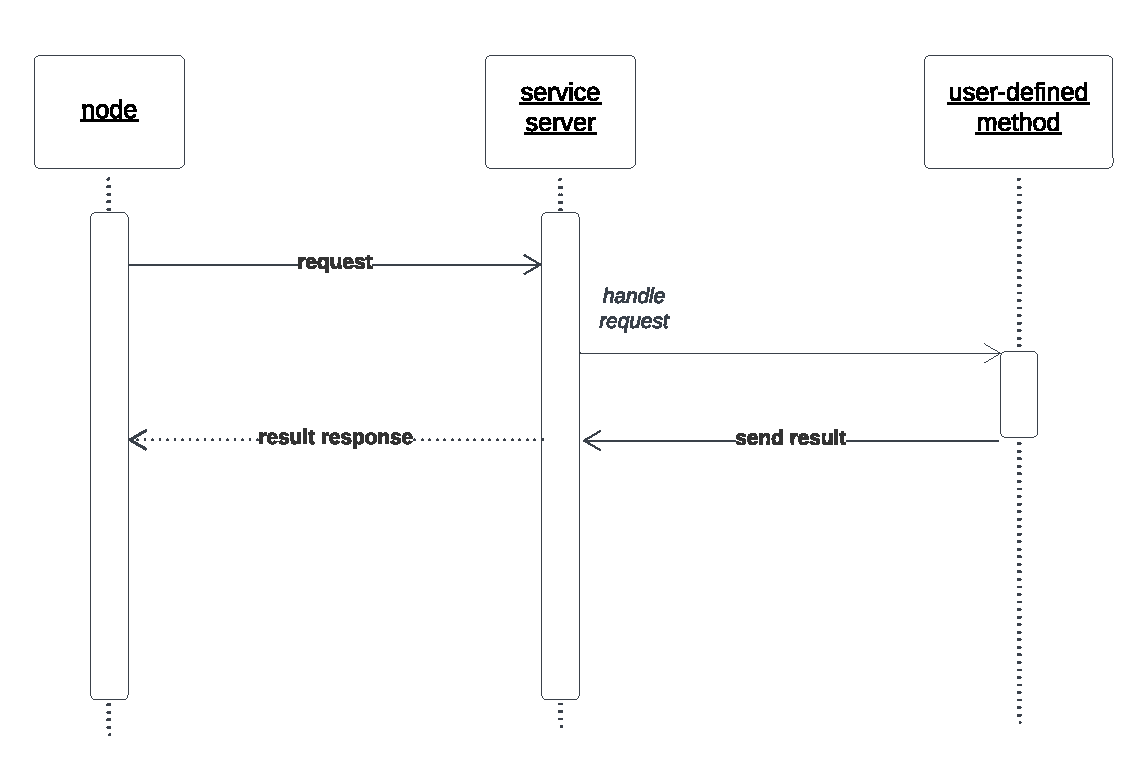
\includegraphics[width=12cm]{figures/lecture4/async_service.pdf}
% \end{center}
% \vspace*{\fill}
% \end{frame}



\subsubsection*{Generation}
\begin{frame}[fragile]{\secsecsec}
\vspace*{\fill}
\begin{center} 
{\mytodo Service Generation} \doublerulefill

\begin{compactitem}
\item \urllink{https://docs.ros.org/en/galactic/Tutorials/Beginner-Client-Libraries/Custom-ROS2-Interfaces.html}{Custom ROS2 Interfaces}:
\begin{compactitem}
\item Add the following in \myfileFoot{CMakeLists.txt}
\begin{cmakescript}
find_package(std_msgs REQUIRED)
find_package(rosidl_default_generators REQUIRED)

set(srv_files
  "srv/AddTwoInts.srv"
)


rosidl_generate_interfaces(${PROJECT_NAME}
  ${srv_files}

  DEPENDENCIES
  builtin_interfaces
  std_msgs
)

ament_export_dependencies(rosidl_default_runtime)
\end{cmakescript}
\end{compactitem}

\end{compactitem}
\end{center}
\vspace*{\fill}
\end{frame}


%%%%%%%%%%%%%%%%%%%%%%%%%%%%%%%%%%%
\begin{frame}[fragile]{\secsecsec}
\vspace*{\fill}
\begin{center} 
{\mytodo Service Generation} \doublerulefill

\begin{compactitem}
\item \urllink{https://docs.ros.org/en/galactic/Tutorials/Beginner-Client-Libraries/Custom-ROS2-Interfaces.html}{Custom ROS2 Interfaces}:
\begin{compactitem}
\item Add the following in \myfileFoot{package.xml}
\begin{xmlscript}
<buildtool_depend>rosidl_default_generators</buildtool_depend>
<exec_depend>rosidl_default_runtime</exec_depend>
<depend>builtin_interfaces</depend>
<depend>std_msgs</depend>  

<member_of_group>rosidl_interface_packages</member_of_group>
\end{xmlscript} 
\end{compactitem}
\end{compactitem}
\end{center}
\vspace*{\fill}
\end{frame}


\begin{frame}[fragile]{\secsecsec}
\vspace*{\fill}
\begin{center} 
{\mytodo Generate Code for the Service} \doublerulefill

\begin{compactenum}
    \item Generate code for the Service:
    \begin{compactitem}
        \item \myTerminal{colcon build -{}-packages-select enpm663_msgs}
    \end{compactitem}
    \item Check related code has been generated in \myFolder{install}
    \item Check the custom Service can be found:
    \begin{compactitem}
        \item \myTerminal{ros2 interface show enpm663_msgs/srv/AddTwoInts}
        \end{compactitem}
\end{compactenum}
\end{center}
\vspace*{\fill}
\end{frame}


\subsubsection*{Server}
%#####################################
\begin{frame}[fragile]{\secsecsec}
\vspace*{\fill}
\begin{center} 

{\mytodo Write the Service Server} \doublerulefill

\vspace{10pt}
\begin{compactitem}
\small
    
    \begin{tabular}{ l l}
    \footnotesize
    {\footnotesize Package} & \myROSPackage{interface_demo} \\
    {\footnotesize Files \raisebox{\dimexpr-\height+8pt}{
\includegraphics[height=9pt, width=9pt]{figures/icons/cpp.png}}} & \myFile{service_server_demo.cpp} and \myFile{service_server_demo.hpp} \\
    {\footnotesize Node} & \myNode{server_demo} \\
    {\footnotesize Executable \raisebox{\dimexpr-\height+8pt}{
\includegraphics[height=9pt, width=9pt]{figures/icons/cpp.png}}} & \myExe{server_demo_exe}\\
    \end{tabular} 

\end{compactitem}

{\mytodo Run the Server} \doublerulefill

\begin{compactitem}
\footnotesize
\item \myTerminal{ros2 run interface_demo server_demo_exe}
\item List all services: \myTerminal{ros2 service list}
\item Message type for the service: \myTerminal{ros2 service type /add_two_ints}
\end{compactitem}

{\mynote} \doublerulefill

\emph{Only an example of a \CC server is provided. Students can see these \urllink{https://docs.ros.org/en/foxy/Tutorials/Beginner-Client-Libraries/Writing-A-Simple-Py-Service-And-Client.html\#write-the-service-node}{instructions} to write a Python server.}
\end{center}
\vspace*{\fill}
\end{frame}


\subsubsection*{Client}
%#####################################
\begin{frame}[fragile]{\secsecsec}
\vspace*{\fill}
\begin{center} 
{\mytodo Use the Service} \doublerulefill

\begin{compactenum}
\footnotesize
    % \item \CC and Python classes were generated from the \myFile{AddTwoInts.srv}
    \item To be able to use this Service in your code you need to:
    \begin{compactitem}
        \item Add the package \myROSPackage{enpm663_msgs} as a dependency.
        \item Include/import header file/module in your code.
    \end{compactitem}
\end{compactenum}

{\faIcon{python}} \doublerulefill

\begin{pyscriptII}
from enpm663_msgs.srv import AddTwoInts
\end{pyscriptII}

{\raisebox{\dimexpr-\height+8pt}{
\includegraphics[height=10pt, width=10pt]{figures/icons/cpp.png}}} \doublerulefill

\begin{cppscriptII}
#include "enpm663_msgs/srv/add_two_ints.hpp"
\end{cppscriptII}

\begin{cmakescript}
find_package(enpm663_msgs REQUIRED)

# Server
add_executable(server_demo_exe src/service_server_demo.cpp)
ament_target_dependencies(server_demo_exe rclcpp enpm663_msgs)

# Client
add_executable(client_demo_exe src/service_client_demo.cpp)
ament_target_dependencies(client_demo_exe rclcpp enpm663_msgs)
\end{cmakescript}

\begin{xmlscriptII}
<depend>enpm663_msgs</depend>
\end{xmlscriptII}

\end{center}
\vspace*{\fill}
\end{frame}


%#####################################
\begin{frame}[fragile]{\secsecsec}
\vspace*{\fill}
\begin{center} 

{\mytodo Write the Service Client} \doublerulefill

\vspace{10pt}
\begin{compactitem}
\small
    
    \begin{tabular}{ l l}
    \footnotesize
    {\footnotesize Package} & \myROSPackage{interface_demo} \\
    {\footnotesize Files \raisebox{\dimexpr-\height+8pt}{
\includegraphics[height=9pt, width=9pt]{figures/icons/cpp.png}}} & \myFile{service_client_demo.cpp} and \myFile{service_client_demo.hpp} \\
    {\footnotesize Files \faIcon{python}} & \myFile{interface_demo.py} \\
    {\footnotesize Node \raisebox{\dimexpr-\height+8pt}{
\includegraphics[height=9pt, width=9pt]{figures/icons/cpp.png}}} & \myNode{client_demo_cpp} \\
    {\footnotesize Node \faIcon{python}} & \myNode{client_demo_py} \\
    {\footnotesize Executable \raisebox{\dimexpr-\height+8pt}{
\includegraphics[height=9pt, width=9pt]{figures/icons/cpp.png}}} & \myExe{client_demo_exe}\\
    {\footnotesize Executable \faIcon{python}} & \myExe{client_demo_exe.py}\\
    \end{tabular} 

\end{compactitem}

{\mytodo Run the Client} \doublerulefill

\begin{compactitem}
\item \raisebox{\dimexpr-\height+9pt}{
\includegraphics[height=10pt, width=10pt]{figures/icons/cpp.png}} \myTerminal{ros2 run interface_demo client_demo_exe}
\item \faIcon{python} \myTerminal{ros2 run interface_demo client_demo_exe.py}
\end{compactitem}

\end{center}
\vspace*{\fill}
\end{frame}


%#####################################
\begin{frame}[fragile]{\secsecsec}
\vspace*{\fill}
\begin{center} 

{\mydefinition Service Call with CLI} \doublerulefill

\emph{You can call services with \myTerminalBlank{ros2 service call}}

\begin{compactitem}
    \small
\item Example: \myTerminal{ros2 service call /add_two_ints  enpm663_msgs/srv/AddTwoInts "\{a: 2 , b: 4\}" }
\end{compactitem}
\end{center}
\vspace*{\fill}
\end{frame}




%%%%%%%%%%%%%%%%%%
%   --- FRAME
%%%%%%%%%%%%%%%%%%
\section{Next Class}
\begin{frame}[fragile]{\sec}
\vspace*{\fill}
\begin{center} 
\Large

\myinfo~\cnordZero{L5:} Knowledge Representation.

\begin{itemize}
\normalsize
    \item We will finish lecture 5.
\end{itemize}

{\large \mywarning Quiz on L5} \doublerulefill

{\large \mywarning Read ARIAC Documentation} \doublerulefill

{\large \mywarning Assignment} \doublerulefill
\end{center}
\vspace*{\fill}
\end{frame}
%=+=+=+=+=+=+=+=+=+=+=+=+=+=+=+=+=+=+=+=+=+=+=+=+=+=+=+=+=+=+=+=+=+=+=+=+=+=+=+=
% END OF DOCUMENT
%=+=+=+=+=+=+=+=+=+=+=+=+=+=+=+=+=+=+=+=+=+=+=+=+=+=+=+=+=+=+=+=+=+=+=+=+=+=+=+=
\end{document}